% ---------------------------------------------------------------------------------------------------------------
% TEMPLATE PARA TRABALHO DE CONCLUSÃO DE CURSO
% Universidade Tecnológica Federal do Paraná - UTFPR
% Customização da classe abnTeX2 (http://www.abntex.net.br/) para as normas da UTFPR
%
% Projeto hospedado em: <link git>
% Autores: Diego Marczal  <>
% 	   Michael Vornes <https://github.com/mvornes>
%
%----------------------------------------------------------------------------------------------------------------
% Codificação: UTF-8
% LaTeX:  abnTeX2          
% ---------------------------------------------------------------------------------------------------------------


% CARREGA CLASSE PERSONALIZADA DA UTFPR--------------------------------------------------------------------------
\documentclass[%twoside,                   % Impressão em frente e verso
    	        oneside,                   % Impressão apenas frente
]{configuracoes/utfpr-abntex2}


% INCLUI ARQUIVOS DE CONFIGURAÇÕES-------------------------------------------------------------------------------
% REFERÊNCIAS------------------------------------------------------------------
\usepackage[%
    alf,
    abnt-emphasize=bf,
    bibjustif,
    recuo=0cm,
    abnt-url-package=url,       % Utiliza o pacote url
    abnt-refinfo=yes,           % Utiliza o estilo bibliográfico abnt-refinfo
    abnt-etal-cite=3,
    abnt-etal-list=3,
    abnt-thesis-year=final
]{abntex2cite}                  % Configura as citações bibliográficas conforme a norma ABNT

% PACOTES----------------------------------------------------------------------
\usepackage[utf8]{inputenc}                                 % Codificação do documento
\usepackage[T1]{fontenc}                                    % Seleção de código de fonte
\usepackage{booktabs}                                       % Réguas horizontais em tabelas
\usepackage{color, colortbl}                                % Controle das cores
\usepackage{float}                                          % Necessário para tabelas/figuras em ambiente multi-colunas
\usepackage{graphicx}                                       % Inclusão de gráficos e figuras
\usepackage{icomma}                                         % Uso de vírgulas em expressões matemáticas
\usepackage{indentfirst}                                    % Indenta o primeiro parágrafo de cada seção
\usepackage{microtype}                                      % Melhora a justificação do documento
\usepackage{multirow, array}                                % Permite tabelas com múltiplas linhas e colunas
\usepackage{subeqnarray}                                    % Permite subnumeração de equações
\usepackage{lastpage}                                       % Para encontrar última página do documento
\usepackage{verbatim}                                       % Permite apresentar texto tal como escrito no documento, ainda que sejam comandos Latex
\usepackage{amsfonts, amssymb, amsmath}                     % Fontes e símbolos matemáticos
\usepackage[algoruled, portuguese]{algorithm2e}             % Permite escrever algoritmos em português
%\usepackage[scaled]{helvet}                                % Usa a fonte Helvetica
\usepackage{times}                                          % Usa a fonte Times
%\usepackage{palatino}                                      % Usa a fonte Palatino
%\usepackage{lmodern}                                       % Usa a fonte Latin Modern
\usepackage[bottom]{footmisc}                               % Mantém as notas de rodapé sempre na mesma posição
\usepackage{ae, aecompl}                                    % Fontes de alta qualidade
\usepackage{latexsym}                                       % Símbolos matemáticos
\usepackage{lscape}                                         % Permite páginas em modo "paisagem"
%\usepackage{picinpar}                                      % Dispor imagens em parágrafos
%\usepackage{scalefnt}                                      % Permite redimensionar tamanho da fonte
%\usepackage{subfig}                                        % Posicionamento de figuras
%\usepackage{upgreek}                                       % Fonte letras gregas

% Redefine a fonte para uma fonte similar a Arial (fonte Helvetica)
\renewcommand*\familydefault{\sfdefault}

% CONFIGURAÇÕES DE APARÊNCIA DO PDF FINAL--------------------------------------
\makeatletter
\hypersetup{%
    portuguese,
    colorlinks=true,   % true: "links" coloridos; false: "links" em caixas de texto
    linkcolor=blue,    % Define cor dos "links" internos
    citecolor=blue,    % Define cor dos "links" para as referências bibliográficas
    filecolor=blue,    % Define cor dos "links" para arquivos
    urlcolor=blue,     % Define a cor dos "hiperlinks"
    breaklinks=true,
    pdftitle={\@title},
    pdfauthor={\@author},
    pdfkeywords={abnt, latex, abntex, abntex2}
}
\makeatother

% ALTERA O ASPECTO DA COR AZUL--------------------------------------------------
\definecolor{blue}{RGB}{41,5,195}

% REDEFINIÇÃO DE LABELS---------------------------------------------------------
\renewcommand{\algorithmautorefname}{Algoritmo}
\def\equationautorefname~#1\null{Equa\c c\~ao~(#1)\null}

% CRIA ÍNDICE REMISSIVO---------------------------------------------------------
\makeindex

% HIFENIZAÇÃO DE PALAVRAS QUE NÃO ESTÃO NO DICIONÁRIO---------------------------
\hyphenation{%
    qua-dros-cha-ve
    Kat-sa-gge-los
}



% INCLUI ARQUIVOS DO TRABALHO DE CONCLUSÃO DE CURSO (PRÉ-TEXTUAIS, TEXTUAIS, PÓS-TEXTUAIS)-----------------------

% INSERE CAPA E FOLHA DE ROSTO
% CAPA---------------------------------------------------------------------------------------------------

% ORIENTAÇÕES GERAIS-------------------------------------------------------------------------------------
% Caso algum dos campos não se aplique ao seu trabalho, como por exemplo,
% se não houve coorientador, apenas deixe vazio.
% Exemplos: 
% \coorientador{}
% \departamento{}

% DADOS DO TRABALHO--------------------------------------------------------------------------------------
\titulo{Sistema \textit{open-source} para a atualização de \textit{firmware} OTA(\textit{Over-The-Air}) baseado nas bibliotecas LwIP, MbedTSL e FatFs}
\titleabstract{Open-Source system for firmware OTA (Over-The-Air) update based on the libraries LwIP, MbedTLS and FatFS}
\autor{Gustavo Luiz Andrade Corrêa}
\autorcitacao{CORRÊA, Gustavo L. Andrade} % Sobrenome em maiúsculo
\local{Pato Branco}
\data{2019}

% NATUREZA DO TRABALHO-----------------------------------------------------------------------------------
% Opções: 
% - Trabalho de Conclusão de Curso (se for Graduação)
% - Dissertação (se for Mestrado)
% - Tese (se for Doutorado)
% - Projeto de Qualificação (se for Mestrado ou Doutorado)
\projeto{Proposta de Trabalho de Conclusão de Curso}

% TÍTULO ACADÊMICO---------------------------------------------------------------------------------------
% Opções:
% - Bacharel ou Tecnólogo (Se a natureza for Trabalho de Conclusão de Curso)
% - Mestre (Se a natureza for Dissertação)
% - Doutor (Se a natureza for Tese)
% - Mestre ou Doutor (Se a natureza for Projeto de Qualificação)
\tituloAcademico{Bacharel}

% ÁREA DE CONCENTRAÇÃO E LINHA DE PESQUISA---------------------------------------------------------------
% Se a natureza for Trabalho de Conclusão de Curso, deixe ambos os campos vazios
% Se for programa de Pós-graduação, indique a área de concentração e a linha de pesquisa
\areaconcentracao{}
\linhapesquisa{}

% DADOS DA INSTITUIÇÃO-----------------------------------------------------------------------------------
% Se a natureza for Trabalho de Conclusão de Curso, coloque o nome do curso de graduação em "programa"
% Formato para o logo da Instituição: \logoinstituicao{<escala>}{<caminho/nome do arquivo>}
\instituicao{Universidade Tecnológica Federal do Paraná}
\departamento{DAINF - Departamento Acadêmico de Informática }
\programa{Curso de Graduação em Engenharia de Computa\c{c}\~ao}
\logoinstituicao{0.2}{dados/figuras/logo-instituicao.png} 

% DADOS DOS ORIENTADORES---------------------------------------------------------------------------------
\orientador{Prof. Dr. Gustavo Weber Denardin}
%\orientador[Orientadora:]{Nome da orientadora}
\instOrientador{Departamento Acadêmico De Elétrica }

\coorientador{}
%\coorientador[Coorientadora:]{Nome da coorientadora}
\instCoorientador{}

% FOLHA DE ROSTO--------------------------------------------------------------------------------------------------------

% TRABALHO DE CONCLUSÃO DE CURSO
 \preambulo{{\imprimirprojeto} apresentado ao {\imprimirprograma} da {\imprimirinstituicao}, como requisito parcial para a obtenção do título de engenheiro de computação.}%{\imprimirtituloAcademico}

% DISSERTAÇÃO DE MESTRADO
% \preambulo{{\imprimirprojeto} apresentada ao Programa de \mbox{Pós-graduação} da {\imprimirinstituicao}, como requisito parcial para obtenção do título de {\imprimirtituloAcademico}.}

% TESE DE DOUTORADO
% \preambulo{{\imprimirprojeto} apresentada ao Programa de \mbox{Pós-graduação} da {\imprimirinstituicao}, como requisito parcial para a obtenção do título de {\imprimirtituloAcademico}.}

% PROJETO DE QUALIFICAÇÃO DE MESTRADO OU DOUTORADO
%\preambulo{{\imprimirprojeto} apresentado ao Programa de \mbox{Pós-graduação} da {\imprimirinstituicao}, como requisito parcial para a obtenção do título de {\imprimirtituloAcademico}.}

% OBSERVAÇÕES-----------------------------------------------------------------------------------------------------------
% Altere este arquivo APENAS comentando as linhas que não se aplicam ao tipo de trabalho acadêmico desejado.


%\usepackage[shortlabels]{enumitem}
\newcommand{\bootloader}{\textit{bootloader}}
\newcommand{\software}{\textit{software}}
\newcommand{\firmware}{\textit{firmware}}
\newcommand{\linker}{\textit{linker}}
\newcommand{\download}{\textit{download}}
\newcommand{\boot}{\textit{boot}}
\newcommand{\resetv}{\textit{reset vector}}
\newcommand{\loader}{\textit{loader}}
\newcommand{\stackp}{\textit{stack pointer}}
\newcommand{\hash}{\textit{hash}}

\begin{document}

\pretextual
\imprimircapa                                               	           % Comando para imprimir Capa
\imprimirfolhaderosto{}                                     		   % Comando para imprimir Folha de rosto
% INSERE ELEMENTOS PRÉ-TEXTUAIS
%% DEDICATÓRIA------------------------------------------------------------------

\renewcommand{\dedicatorianame}{DEDICATÓRIA}

\begin{dedicatoria}

Altere este texto inserindo a dedicatória do seu trabalho. 

\end{dedicatoria}
          			   % Dedicatória
%% AGRADECIMENTOS---------------------------------------------------------------

\begin{agradecimentos}[AGRADECIMENTOS]

Edite e coloque aqui os agradecimentos às pessoas e/ou instituições que contribuíram para a realização do trabalho.

É obrigatório o agradecimento às instituições de fomento à pesquisa que financiaram total ou parcialmente o trabalho, inclusive no que diz respeito à concessão de bolsas.

\end{agradecimentos}
        			   % Agradecimentos
%% EPÍGRAFE---------------------------------------------------------------------

\renewcommand{\epigraphname}{EPÍGRAFE}

\begin{epigrafe}

\textit{Technology is just nature we taught to do cool tricks. (EXURB1A, 2019)
}

\end{epigrafe}

% OBSERVAÇÕES------------------------------------------------------------------
% Altere o texto para inserir a epígrafe do seu trabalho

              			   % Epígrafe
% RESUMO--------------------------------------------------------------------------------

\begin{resumo}[RESUMO]
\begin{SingleSpacing}

% Não altere esta seção do texto--------------------------------------------------------
\imprimirautorcitacao. \imprimirtitulo. \imprimirdata. \pageref {LastPage} f. \imprimirprojeto\ – \imprimirdepartamento, \imprimirinstituicao. \imprimirlocal, \imprimirdata.\\
%---------------------------------------------------------------------------------------


Com a ampla utilização  de internet das coisas, conceito em que dispositivos embarcados estão conectados a internet, surge a necessidade da atualização automática do \textit{firmware} desses dispositivos para correções ou aperfeiçoamentos. Atualmente existem uma grande variedade de implementações dessa funcionalidade, mas a falta de um padrão dificulta a sua ampla utilização.
Assim, esse trabalho propõe uma solução \textit{open-source} de atualização de \textit{firmware Over-The-Air} para dispositivos IoT, utilizando as bibliotecas amplamente difundidas LwIP, FatFs e Mbed TLS.
O sistema pretende proposto disponibilizar uma API, que pode ser integrada a qualquer plataforma embarcada, que irá obter o novo \textit{firmware} de um servidor, e um \textit{bootloader} que faz todo o processo de troca do \textit{firmware}.


\textbf{Palavras-chave}: Atualização. Firmware. Over-The-Air. Portável. IoT.

%O Resumo é um elemento obrigatório em tese, dissertação, monografia e TCC, constituído de uma seqüência de frases concisas e objetivas, fornecendo uma visão rápida e clara do conteúdo do estudo. O texto deverá conter no máximo 500 palavras e ser antecedido
%pela referência do estudo. Também, não deve conter citações. O resumo deve ser redigido em parágrafo único, espaçamento simples e seguido das palavras representativas do conteúdo do estudo, isto é, palavras-chave, em número de três a cinco, separadas entre si por ponto e finalizadas também por ponto. Usar o verbo na terceira pessoa do singular, com linguagem impessoal, bem como fazer uso, preferencialmente, da voz ativa. Texto contendo um único parágrafo.\\



\end{SingleSpacing}
\end{resumo}

% OBSERVAÇÕES---------------------------------------------------------------------------
% Altere o texto inserindo o Resumo do seu trabalho.
% Escolha de 3 a 5 palavras ou termos que descrevam bem o seu trabalho 

             			   % Resumo em Português
%% ABSTRACT--------------------------------------------------------------------------------

\begin{resumo}[ABSTRACT]
\begin{SingleSpacing}

% Não altere esta seção do texto--------------------------------------------------------
\imprimirautorcitacao. \imprimirtitleabstract. \imprimirdata. \pageref {LastPage} f. \imprimirprojeto\ – \imprimirprograma, \imprimirinstituicao. \imprimirlocal, \imprimirdata.\\
%---------------------------------------------------------------------------------------

Elemento obrigatório em tese, dissertação, monografia e TCC. É a versão do resumo em português para o idioma de divulgação internacional. Deve ser antecedido pela referência do estudo. Deve aparecer em folha distinta do resumo em língua portuguesa e seguido das palavras representativas do conteúdo do estudo, isto é, das palavras-chave. Sugere-se a elaboração do resumo (Abstract) e das palavras-chave (Keywords) em inglês; para resumos em outras línguas, que não o inglês, consultar o departamento / curso de origem.\\

\textbf{Keywords}: Word. Second Word. Another word.

\end{SingleSpacing}
\end{resumo}

% OBSERVAÇÕES---------------------------------------------------------------------------
% Altere o texto inserindo o Abstract do seu trabalho.
% Escolha de 3 a 5 palavras ou termos que descrevam bem o seu trabalho 
             		           % Resumo em Inglês
% Lista de Figuras----------------------------------------------------------------

\pdfbookmark[0]{\listfigurename}{lof}
\listoffigures*
\cleardoublepage

% OBSERVAÇÕES---------------------------------------------------------------------
% Este arquivo não precisa de ser alterado, pois a lista é gerada automaticamente.
   % Lista de Figuras
%% LISTA DE QUADROS----------------------------------------------------------------

\renewcommand{\listofquadrosname}{LISTA DE QUADROS}

\pdfbookmark[0]{\listofquadrosname}{loq}
\listofquadros*
\cleardoublepage

% OBSERVAÇÕES---------------------------------------------------------------------
% Este arquivo não necessita de ser editado. A lista é gerada automaticamente.
   % Lista de Quadros
% LISTA DE TABELAS-------------------------------------------------------------

\pdfbookmark[0]{\listtablename}{lot}
\listoftables*
\cleardoublepage

% OBSERVAÇÕES-------------------------------------------------------------------
% Este arquivo não precisa ser alterado, pois a lista é gerada automaticamente.
         		   % Lista de Tabelas
%% LISTA DE ABREVIATURAS E SIGLAS----------------------------------------------------------

\begin{siglas}
    \item[API] Application Programming Interface 
    \item[CAN] Controller Area Network
    \item[FAT]  File Allocation Table
    \item[HAL] Hardware Abstraction Layer
    \item[HTTP] Hypertext Transfer Protocol
    \item[HTTPS]  Hypertext Transfer Protocol Secure
    \item[I2C] Inter-Integrated Circuit
    \item[IoT] Internet of things
    \item[IP] Internet Protocol 
    \item[OTA] Over-The-Air 
    \item[RAM] Random Access Memory  
    \item[ROM] Read Only Memory
    \item[RTOS] Real-Time Operating System
    \item[SD] Secure Digital
    \item[SHA] Secure Hash Algorithm
    \item[SPI] Serial Peripheral Interface
    \item[SSL]  Secure Sockets Layer
    \item[TCP] Transmission Control Protocol 
    \item[TLS] Transport Layer Security
    \item[UART] Universal asynchronous Receiver-Transmitter
    \item[USB] Universal Serial Bus


      
\end{siglas}

% OBSERVAÇÕES-----------------------------------------------------------------------------
% Altere a lista acima para definir os acrônimos e siglas utilizados neste trabalho
          		   % Lista de Abreviaturas e Siglas
%% LISTA DE SÍMBOLOS------------------------------------------------------------

\begin{simbolos}
    \item[$ \Gamma $] Letra grega Gama
    \item[$ \lambda $] Comprimento de onda
    \item[$ \in $] Pertence
\end{simbolos}

% OBSERVAÇÕES-------------------------------------------------------------------
% Altere a lista acima para definir os símbolos utilizados no trabalho
        		   % Lista de Símbolos
%% LISTA DE ALGORITMOS----------------------------------------------------------

\newcommand{\algoritmoname}{Algoritmo}
\renewcommand{\listalgorithmcfname}{LISTA DE ALGORITMOS}

\floatname{algocf}{\algoritmoname}
\newlistof{listofalgoritmos}{loa}{\listalgoritmoname}
\newlistentry{algocf}{loa}{0}

\counterwithout{algocf}{chapter}
\renewcommand{\cftalgocfname}{\algoritmoname\space}
\renewcommand*{\cftalgocfaftersnum}{\hfill--\hfill}

\pdfbookmark[0]{\listalgorithmcfname}{loa}
\listofalgorithms
\cleardoublepage

% OBSERVAÇÕES------------------------------------------------------------------
% Este arquivo não precisa ser alterado, pois a lista é gerada automaticamente.
   % Lista de Algoritmos
% SUMÁRIO----------------------------------------------------------------------

\renewcommand{\contentsname}{SUMÁRIO}

\pdfbookmark[0]{\contentsname}{toc}
\tableofcontents*
\cleardoublepage

% OBSERVAÇÕES-------------------------------------------------------------------
% Este arquivo não precisa ser alterado, pois o sumário é gerado automaticamente.
               			   % Sumário

\textual
% INSERE ELEMENTOS TEXTUAIS
% INTRODUÇÃO-------------------------------------------------------------------

\chapter{INTRODUÇÃO}
\label{chap:introducao}
Com a evolução da microeletrônica e, por consequência, a redução de custo de periféricos e o crescimento do poder computacional de processadores, os sistemas computacionais se tornaram menores e baratos. Devido a isso, processadores e microcontroladores passaram a ser instalados em produtos, o que deu origem ao conceito de sistema embarcado, que são sistemas de processamento de informação embutidos em produtos \cite{Marwedel2006}.
A utilização desses sistemas foi disseminada em várias áreas como, a automobilística, aeronáutica, ferroviária, industrial, médica, entre outras, automatizando as mais diversas funções. 
%Em algumas dessas funções era fundamental a presença de agentes humanos para serem realizadas, ou não existiam, pois, uma pessoa não a exerceria em tempo hábil.

% \textit{Apollo Guidance Computer} (AGC) foi conhecido como o primeiro sistema embarcado da história, instalado no \textit{Apollo command module} e no \textit{Apollo Lunar Module}, tinha como proposito principal fornecer interfaces eletrônicas e de computação para orientação, navegação e controle da espaçonave.


Os sistemas computacionais embarcados são compostos pelos mesmos componentes utilizados para a constituição de computadores pessoais, porém com tamanhos, capacidades e custos reduzidos. Tais dispositivos operam de forma independente e geralmente são projetados para realizar tarefas específicas e repetitivas. 
Sistemas embarcados estão presentes no dia a dia da maioria das pessoas, em micro-ondas, geladeiras, TVs, aparelhos de som, video games e outros produtos eletrônicos \cite{Marwedel2006}, logo, esses dispositivos se distanciam dos computadores de propósito geral, como observamos em \textit{desktops} e \textit{notebooks} atuais. 
%CORRIGIR automatizando diversas funções, estas que anteriormente eram fundamental a presença de agentes humanos para serem realizadas. 

%a manutenção desses sistemas não é algo banal, e por vezes esquecida durante a faze de projeto destes produtos,



Com a necessidade cada vez maior da implementação desses sistemas no nosso dia a dia, é imprescindível se obter \textit{hardwares} e \textit{softwares}, cada vez mais robustos e que atendam todas as necessidades dos seus usuários.
Assim, o projeto desses produtos devem ser muito bem planejado, e executado de forma a serem entregues produtos de qualidade, à  prova de falhas e que possam reagir a erros, de forma a não causar danos a seus utilizadores. 
%Os \textit{software}s desenvolvidos para sistemas embarcados muitas vezes são chamados de \textit{firmware}.
%e como um desenvolvimento completamente sem falhas, \textit{bugs} e com máxima eficiência é quase inconcebível

%Alguns \textit{software}s produzidos para projetos de larga e pequena escala acabam por chegar em seus consumidores finais pouco otimizados e até mesmo com erros, fazendo com que isto gere desconforto, perda de valor, e em casos extremos a morte de usuários. Como mostrado pelo relatório do Barr Group 


%Pensando na durabilidade e qualidade destes produtos,
Durante a fase de projeto de um sistema embarcado, deve-se avaliar diversos âmbitos, como desempenho, confiabilidade, consumo de energia, manufaturabilidade, etc. É também necessário validar essas avaliações, com o intuito de verificar se atenderão os requisitos de projeto. Pela necessidade desses produtos serem eficientes, é indispensável que esses sistemas passem por uma fase de otimização, em que mudanças no projeto podem melhorar a eficiência energética do produto ou até mesmo gerar novas funcionalidades a esses equipamentos. Portanto, o projeto todo precisa ser testado para evitar que erros e \textit{bugs} possam vir a permanecer no produto final \cite{Marwedel2006}, criando um ciclo de desenvolvimento que deve ser repetido até se obter um produto eficiente, de qualidade e completo.
%Por vezes as manutenções futuras do \textit{firmware} é esquecida, ou então ignorada, durante a fase de projeto, até por que esta é cara e não é algo banal, principalmente em projetos já implantados.

Após a venda e instalação de um sistema embarcado para seu cliente, eventualmente pode ser necessária uma nova funcionalidade, uma otimização ou então, podem ser exigidos testes nesse sistema. Logo, é preciso que haja uma forma de se alterar esse produto mesmo após seu lançamento, para assim darmos um maior valor ao produto e confiabilidade ao sistema.
A possibilidade de serem feitas manutenções futuras no \textit{software}, que no contexto de sistemas embarcados é chamado de \textit{firmware} (\textit{firmware} é uma classe específica de \textit{software} de computador que fornece controle de baixo nível para o \textit{hardware} específico do dispositivo), é conhecida como atualização OTA (\textit{Over-The-Air}). Esse recurso não é obrigatório no projeto de um sistema embarcado, mas é muitas vezes necessário, podendo ser uma funcionalidade muito útil dependendo da aplicação do sistema em concepção. A decisão de utilizar ou não a atualização OTA pode influenciar na escolha do \textit{hardware} utilizado no projeto \cite{Ball2002}, 
%também não é tão banal de ser criada, 
podendo aumentar o custo do produto final.
Uma das principais soluções adotadas para a manutenção desses programas é criar métodos de atualização em que, é necessário a presença de um agente humano fisicamente próximo do sistema para fazer a manutenção do \textit{software}, o que acaba aumentando o custo de manutenção do produto e o tornando menos atrativo para os seus compradores.

%Geralmente os sistemas de atualização remotos presentes em sistemas embarcados atuais utilizam ferramentas proprietarias e ...
Os \textit{bootloaders} estão atualmente presentes em todos os computadores pessoais e em alguns sistemas embarcados. Esse \textit{software} prepara a maioria dos \textit{hardwares} presentes na máquina para um sistema operacional ou outro programa ser executado.
Como é o primeiro programa a ser executado após um sistema ser iniciado ou após um \textit{reset}, ele pode ter várias funções, como, realizar checagem de periféricos, verificar se o \textit{firmware} presente na memória não está corrompido, além de poder fazer a troca do \textit{software} presente na memória \cite{DavesDurlin2013}, que será sua principal utilização nesse trabalho.

Um dos seus principais usos é em \textit{smartphones}, em que são utilizados para a atualização de sistemas operacionais como \textit{Android} e iOS, e como garantia de restauração em caso de erros irreversíveis no sistema operacional. É desenvolvido pelo próprio fabricante do dispositivo, e por padrão é bloqueado para os usuários, evitando a substituição do \textit{software} original do aparelho por uma versão customizada, mas ainda assim existem opções de desbloqueio do \textit{bootloader}, dependendo do modelo do aparelho e do fabricante \cite{Salute2018}.% mas pode destravada o \textit{bootloader}.

\textit{Internet of things} ou IoT é o conceito que se refere à interconexão digital de objetos cotidianos com a internet. A internet das coisas em outras palavras pode ser descrita como uma rede de dispositivos embarcados, como sensores, câmeras, carros e demais objetos do cotidiano, capazes de obter e transmitir dados pela internet. Em 2019, a empresa de consultoria Gartner \cite{Gartner} diz que, até 2020, são esperados mais de 20 bilhões de "coisas"\  conectadas a internet. Essas "coisas"\  não são dispositivos de uso geral como \textit{smartphones} e PCs, mas objetos de função única.

Nesse cenário de crescimento constante de dispositivos embarcados conectados a internet, o presente trabalho de conclusão de curso propõe um método de manutenção desses \textit{firmwares} de forma remota, que possa ser o mais portável possível para a família de microcontroladores STM32.
Na solução proposta, o dispositivo embarcado poderá verificar periodicamente um servidor a procura de uma nova versão do seu \textit{firmware}. Quando encontrado, será realizado o \textit{download} do novo \textit{firmware} para a memória interna do dispositivo, para posterior atualização do equipamento. O diferencial da abordagem proposta é basear a solução em bibliotecas amplamente difundidas em sistemas embarcados, como a LwIP \cite{LWIP}, Mbed TLS \cite{mbedtls} e a FatFS\cite{FATFS}. Dessa forma, o código do sistema de atualização é totalmente portável, desde que a plataforma escolhida tenha suporte a tais bibliotecas. A única peça de \textit{software} que não será totalmente portável será o \textit{bootloader} que substituirá o \textit{firmware} antigo pelo novo na memória flash do dispositivo, por ser dependente do \textit{hardware} utilizado.

%O Geovanni marcou o nome das bibliotecas, mas não sei se é para deixar elas em italico.
%Citar Bibliotecas!!!!
 
%para a plataforma STM32F746, onde, através de um servidor na internet, um novo código pode ser enviado ao \textit{hardware}, por uma requisição do próprio sistema embarcado. Existirão tarefas que farão a verificação da disponibilidade da atualização, e o download de forma segura, utilizando as bibliotecas já bem estabelecidas LwIP e MbedTSL, a gravação deste arquivo e do \textit{software} anteriormente instalado no produto, em um cartão SD, para caso haja a necessidade de se reverter a atualização, será feita por meio da biblioteca FatFs, e então a troca do antigo \textit{software} pelo novo é feito a partir de um \textit{bootloader}.






%Falar sobre a utilização de bootloaders em sistemas android em celulares... e citar sites falando sobre bootloaders


%Edite e coloque aqui o seu texto de introdução.

%A Introdução é a parte inicial do texto, na qual devem constar o tema e a delimitação do assunto tratado, objetivos da pesquisa e outros elementos necessários para situar o tema do trabalho, tais como: justificativa, procedimentos metodológicos (classificação inicial), embasamento teórico (principais bases sintetizadas) e estrutura do trabalho, tratados de forma sucinta. Recursos utilizados e cronograma são incluídos quando necessário. Salienta-se que os procedimentos metodológicos e o embasamento teórico são tratados, posteriormente, em capítulos próprios e com a profundidade necessária ao trabalho de pesquisa.

\section{OBJETIVO GERAL}
\label{sec:Objetivo Geral}

Esse trabalho tem como objetivo geral o desenvolvimento de um sistema \textit{open-source} para a atualização  de \textit{firmwares} \textit{Over The Air} para dispositivos IoT baseado nas bibliotecas FatFs, LwIP e Mbed TLS. 

\section{OBJETIVOS ESPECÍFICOS}
\label{sec:Objetivos Específicos}

 \begin{itemize}
   \item Desenvolver o \bootloader\ para microcontroladores STM32 utilizando a biblioteca FatFS..
   
   %\item Criar um servidor HTTP para a comunicação cliente-servidor.
   
   \item Implementar uma API que fará a comunicação segura entre o servidor e a plataforma embarcada, verificará a disponibilidade de atualização e fará o \textit{download} da nova versão, se existente. Ainda, armazenará o \textit{firmware} recebido em um cartão SD (Secure Digital). 
   %terminar essa
   
   %\item Produzir a tarefa de leitura de um cartão micro SD que guarda uma nova versão do \textit{firmware} e uma cópia do anterior, utilizando a biblioteca FatFs.
   %modificar a palavra produzir??
   \item Comprovar o funcionamento da técnica de atualização remota de \textit{firmware}, utilizando a plataforma embarcada STM32F746G-DISCOVERY.
   
 \end{itemize}
 
                		           % Introdução
% REVISÃO DE LITERATURA--------------------------------------------------------

\chapter{REVISÃO DA LITERATURA}
\label{chap:fundamentacaoTeorica}
Neste capítulo será feita uma revisão da literatura necessária para o entendimento deste trabalho de conclusão de curso. 
Serão abordados os temas como: o processo de inicialização de um sistema embarcado, o que é um \bootloader\ e o papel do \linker\ na criação de um arquivo executável e no mapeamento da memória da aplicação.
Também será discutido sobre  a comunicação cliente-servidor, a pilha TCP/IP, a biblioteca LwIP e alguns protocolos implementados por ela, assim como a biblioteca Mbed TLS, alguns protocolos e algoritmos de segurança implementados por ela.
Será mostrado o que é um sistema de arquivo, o sistema de arquivos FAT e a biblioteca FatFs.
Com o conhecimento obtido sobre todos esses temas o leitor será capaz de compreender como será desenvolvido o método de atualização de \firmware\ OTA.


%\section{PLATAFORMA EMBARCADA — STM32F7 DISCOVERY}%materiais
%\section{SISTEMAS EMBARCADOS}
%\subsection{ARM M7 E SUA FAMÍLIA.}
%\section{FIRMWARE OVER THE AIR}
%O conceito de \textit{firmware over the air} (FOTA),  consiste em um mecanismo de atualização remoto de firmware, já é muito utilizado em firmware de smartfones por fornecer uma forma segura, eficiente e conveniente de atualização.geralmente utilizado em smartfones.  
\section{PROCESSO DE INICIALIZAÇÃO DO SISTEMA}

Segundo \citeonline{Qing2003}, um processador embarcado, após ser ligado, busca e executa o código de um endereço pré-definido e gravado permanentemente na memória. O código contido nessa localização da memória é chamado de \resetv. O \resetv\ é usualmente uma instrução de salto para outro espaço da memória em que o real código de inicialização se encontra. A razão deste salto para outra localidade da memória é para manter o \resetv\ pequeno. O \resetv\ pertence a uma pequena área da memória reservada pelo sistema por motivos especiais. O \resetv, assim como o código de inicialização do sistema, precisa estar armazenado permanentemente. Por causa deste problema, o código de inicialização, chamado de código \textit{bootstrap}, reside na memória somente de leitura (ROM), na flash ou em outra memória não volátil. O termo \textit{loader} se refere ao código que é responsável por executar o \textit{bootstrap}, fazer o possível \download\ de uma imagem de outro local e inicialização da aplicação final.

O conceito é melhor explicado por meio de um exemplo. Neste exemplo, iremos assumir que o \loader\ foi desenvolvido e programado na memória flash. Além disso, será assumido que a imagem alvo contém várias seções de programa. Cada seção tem um lugar designado no mapa de memória. O \resetv\ está contido em uma pequena ROM, que está mapeada na localização 0x0h do espaço de endereços. A ROM contém alguns valores iniciais essenciais requeridos pelo processador quando o sistema é reinicializado (\textit{reset}). Esses valores são o \resetv, o \textit{stack pointer} (ponteiro de pilha) inicial e o endereço da memória de acesso randômico (RAM) usável. 

No exemplo ilustrado na \autoref{fig:INICIALIZAÇÃO}, o \resetv\ é uma instrução de salto para o endereço de memória 0x00040h; o \resetv\ transfere o controle do programa para a instrução neste endereço. O código de inicialização do sistema contém, entre outras coisas o programa \loader\ da imagem destino e o vetor de exceção padrão do sistema (\textit{exception vector}). O vetor de exceção do sistema aponta para uma instrução que reside na memória flash.

A primeira parte do processo de \textit{bootstrap} do sistema é colocar o sistema em um estado conhecido. São colocados valores padrões apropriados nos registradores do processador. São colocados no \stackp\ os valores encontrados na ROM. O \loader\ desabilita as interrupções do sistema, pois o sistema ainda não está preparado para lidar com interrupções. O \loader\ também inicializa a memória RAM e possivelmente a \textit{cache} (memória transitória) do processador. Neste ponto, o \loader\ executa um diagnóstico de \textit{hardware} limitado nos dispositivos necessários para essas operações.

A execução do programa é mais rápida na RAM quando comparada ao mesmo código executado diretamente na memória flash. O \loader\ pode opcionalmente copiar o código da memória flash para a RAM. Por causa dessa capacidade, uma seção de programa pode tanto ter um endereço de carregamento, quanto um endereço de execução. O endereço de carregamento é onde a seção do programa reside, enquanto o endereço de execução é o endereço em que o \loader\ copia a seção do programa e a prepara para a execução.

\begin{figure}[H]
    \scriptsize
     \centering
     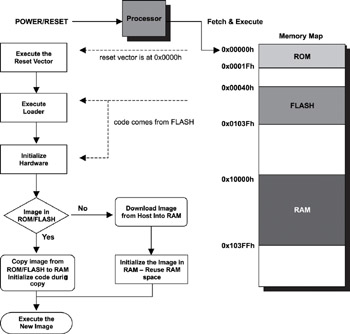
\includegraphics[scale=1]{dados/figuras/BootOriginal.png}
     \caption{Processo de inicialização de um sistema embarcado.\newline Fonte:\cite{Qing2003}}
     \label{fig:INICIALIZAÇÃO}
\end{figure}

Uma imagem executável possui seções de dados inicializados e não inicializados. Essas seções são ambas legíveis e graváveis. Essas seções precisam residir na RAM, assim sendo são copiadas da memória flash para a RAM como parte do sistema de inicialização. A seção de dados inicializados (chamadas pelo \linker\ de .data e .sdata) contém os valores iniciais para as variáveis globais e estáticas. O contéudo dessa seção, portanto, faz parte da imagem executável final e é transferido completamente pelo \loader. Por outro lado, o contéudo da seção de dados não inicializado (chamado pelo \linker\ de .bss e .sbss) é vazio. O \linker\ reserva espaço para essa seção no mapa de memória. As informações de alocação dessas seções, como o tamanho da seção e o endereço de execução da seção, são parte do cabeçalho da seção. É trabalho do \loader\ obter essas informações dos cabeçalhos de seção e alocar a mesma quantidade de memória na RAM durante o processo de carregamento. O \loader\ coloca essas seções na RAM de acordo com o endereço de execução das seções.

Uma imagem executável provavelmente possui constantes. Os dados das contantes são parte da seção chamada pelo \linker\ de .const, que é somente leitura. Sendo assim, é possível manter a seção .const na memória somente de leitura durante a execução do programa. Constantes de acesso frequente, como tabelas de \textit{lookup}, necessitam ser transferidas para a RAM para melhorar o desempenho do sistema.

O próximo passo no processo de inicialização do sistema é o \loader\ inicializar os dispositivos do sistema. Apenas os dispositivos necessários são inicializados nessa etapa. Em outras palavras, um dispositivo é inicializado na medida em que um subconjunto necessário dos recursos e recursos do dispositivo estejam ativados e operacionais. Geralmente, os dispositivos são parte da interface de entrada e saída do sistema, portanto, esses dispositivos são completamente iniciados quando existe a necessidade de se fazer \download\ de uma imagem de outro local.

Agora o \loader\ está pronto para transferir a imagem da aplicação para o sistema alvo. A imagem da aplicação pode conter um RTOS, um \textit{kernel}, e os demais códigos das aplicações que o desenvolvedor necessita.


%Conhecer o processo de inicialização dos sistemas embarcados, também chamado de \boot, é muito importante para nos dar noção sobre quando e como entrará em execução tanto a aplicação final, quanto o bootloader.
%Dependendo do fabricante do \textit{chip} o \boot pode ser diferente, porém geralmente ele segue a mesma linha de execução, podendo ou não ter interfaces físicas para mudar a origem do \boot. Algumas placas da ST \cite{ST2019}, contém um mecanismo chamado de \textit{physic remap}, para que o \boot ocorra a partir de outras memórias e não da Flash, que é a padrão \cite{Noviello2018}.

%Como dito por \citeonline{Beningo2015}, o fluxo padrão de \boot do sistema consiste em, após a tensão de referência de um microcontrolador se estabilizar, o processador procura pelo vetor de \textit{reset}, para a obter a localização da instrução de iniciação na Flash. O vetor de reset esta localizado em um endereço especial da memória FLASH, geralmente no início. Como pode ser visto na imagem \ref{MAP_PIC24F16KLXXX} que contém o mapa de memória do MCU (\textit{microcontroller unit}) PIC24F16KLXXX, o vetor de \textit{reset} se encontra no endereço 0x0002.

%\begin{figure}[H]
 %   \scriptsize
 %    \centering
     %\includegraphics[scale=1]{dados/figuras/%ResetVector.jpg}
     %\caption{Mapa de memória do MCU PIC24F16KLXXX.\newline Fonte: \cite{Beningo2015}}
     %\label{MAP_PIC24F16KLXXX}
%\end{figure}

%Então o endereço contido no vetor de \textit{reset} é carregado pelo microcontrolador, e a instrução contida neste endereço é carregada e executada pelo processador. Essa instrução ainda não é a \textit{main} que foi desenvolvida pelo projetista, ela é somente uma instrução de como o MCU irá iniciar. Esta instrução geralmente tem como função copiar o \textit{Vector Table} que esta na memória FLASH para a RAM, copiando e escrevendo em um endereço determinado pelo arquivo de \linker.

%As variáveis que são inicializadas durante o tempo de compilação que estão armazenadas na seção \textit{.data} do arquivo de \linker são então gravadas na memória RAM, e as variáveis não inicializadas explicitamente ou iniciadas com zero que estão na seção \textit{.bss} do arquivo de \linker, são guardadas na memória RAM. O MCU então copia funções que estão na FLASH para a RAM, essa etapa é opcional, o projetista tem que determinar se alguma função deve necessariamente ser executada a partir da memória RAM. 

%Todo esse processo é chamado de \textit{"C Copy Down"}, que faz a preparação do ambiente para iniciar uma aplicação, após essa etapa ser concluída o MCU pode então chamar a função \textit{main}, que é a \firmware principal do sistema desenvolvido pelo projetista. Toda a sequência padrão de \textit{boot} pode ser observada na \autoref{Seq_Boot}.

%\begin{figure}[H]
 %   \scriptsize
  %   \centering
   %  
\includegraphics[scale=1]{dados/figuras/ToDo.jpg}
    % \caption{Sequencia de Boot.}
     %\label{Seq_Boot}
%\end{figure}

%É possível alterar a função da tarefa contida no vetor de \textit{reset} no arquivo de \linker, fazendo com que o MCU passe pelo processo de \textit{C Copy Down}, preparando o sistema para outra função diferente da aplicação principal do sistema embarcado, como é utilizado na criação de um \bootloader para a atualização de \firmware.













\subsection{BOOTLOADER}

O \bootloader\ é um \textit{software} que tem como responsabilidade a atualização do \firmware\ do sistema, operação também conhecida como \textit{in-aplicattion programing} (IAP). Reside em uma área protegida da memória, geralmente colocado no início da flash ou na ROM, e é o primeiro \textit{software} a ser executado após o \textit{reset} ou iniciação do sistema.
É desenvolvido para receber comandos via periféricos de comunicação como: UART, I2C, SPI, CAN e Ethernet, e entender o mapa de memória do microcontrolador \cite{DavesDurlin2013}. A \autoref{Diag_Bootloader} mostra como geralmente fica alocado um \bootloader\ e o \firmware\ na memória.
% que são usados para trocar do firmware do MCU e recebimento do novo código de aplicação. Frequentemente é necessário um programa externo para dar esses comandos ao bootloader \cite{Noviello2018}.

\begin{figure}[H]
    \scriptsize
     \centering
     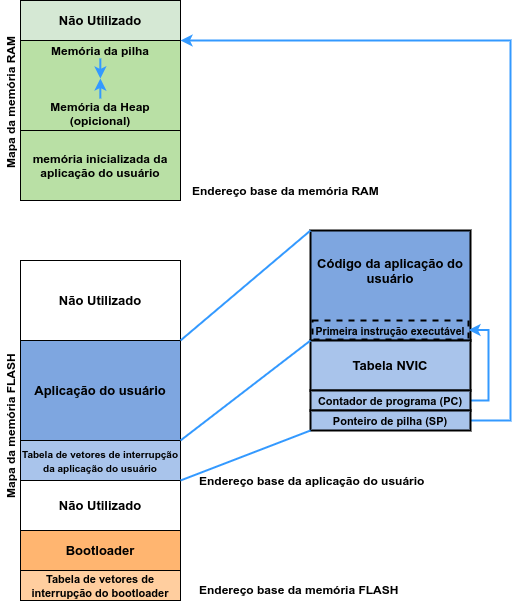
\includegraphics[scale=0.7]{dados/figuras/DiagBootloaderOriginal.png}
     \caption{Alocação do bootloader e firmware nas memórias flash e ram.\newline Fonte:\cite{DavesDurlin2013}}
     \label{Diag_Bootloader}
\end{figure}

Sua função se resume geralmente a: comunicar-se com outro servidor, ler os arquivos enviados pelo \textit{host}, atualizar o \firmware\ de seu microcontrolador, e iniciar esse novo \software. 
Pode conter instruções e comandos definidos pelo projetista para somente o circuito integrado em uso, impossibilitando a utilização do mesmo código em outras placas.
%Sendo desenvolvidos exatamente para o \textit{hardware} que serão empregados,
Portanto, é uma peça de \textit{software} que não é portável para várias plataformas. A \autoref{FluxoBootloader} mostra o funcionamento de um bootloader padrão. 

\begin{figure}[H]
    \scriptsize
     \centering
     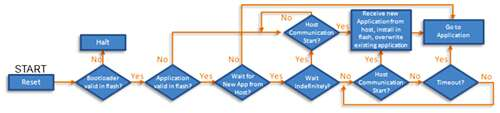
\includegraphics[scale=1]{dados/figuras/FluxoBootloader.jpg}
     \caption{Fluxograma de operações de um bootloader.}
     \label{FluxoBootloader}
\end{figure}



Os sistemas microcontrolados STM32 possuem um \bootloader\ pré programado na ROM desde sua fabricação. Esse \bootloader\ pode utilizar diversos periféricos de comunicação, e para cada periférico diferente a ST padronizou diferentes protocolos que permitem várias operações, como: obter o ID do chip, escrever e ler bytes na RAM e memória flash, apagar setores das memórias, ativar áreas de proteção na memória e pular para o código principal do sistema \cite{Noviello2018}.

É possível ser criado um \bootloader\ customizado com diversas funções adicionais. Uma função frequentemente usada é o uso do \bootloader\ para descriptografar firmwares que podem chegar via internet, para se garantir a segurança e origem do \firmware, assim após esse processo o sistema pode substituir o \software\ anterior pelo recebido. 



\subsection{LINKER}

Segundo \citeonline{Qing2003}, os arquivos de uma aplicação são processados pelo compilador e \textit{assembler}. Criando assim os arquivos objetos, que contém os códigos de máquina binários (\textit{machine binary code}) e dados de programa (\textit{program data}). O \textit{archive utility} concatena uma coleção de arquivos objetos para formar uma biblioteca. Então o \linker\ obtém esses arquivos objetos como entrada e produz ou um arquivo executável, ou um arquivo objeto que pode ser utilizado em outro \linker\ com outros arquivos objetos. O arquivo de comandos de \linker\ (\textit{linker command file}) orienta o \linker\ em como combinar esses diferentes arquivos objetos e aonde colocar o código binário e os dados no sistema embarcado alvo. Assim podemos concluir que, a função principal de um \linker\ é combinar múltiplos arquivos objetos em um arquivo objeto relocável maior, um arquivo objeto compartilhado ou uma imagem executável final. Esse processo pode ser observado na \autoref{linker}.

\begin{figure}[H]
    \scriptsize
     \centering
     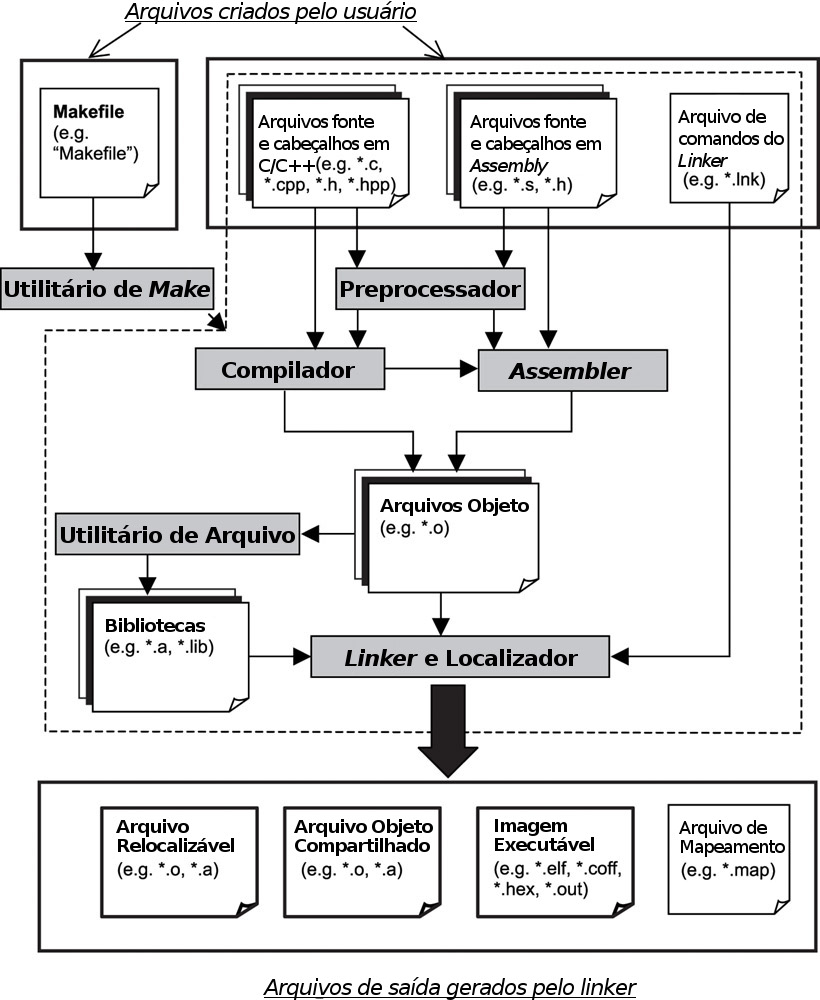
\includegraphics[scale=0.5]{dados/figuras/Linker.png}
     \caption{Criando um arquivo de imagem para um sistema alvo.\newline Fonte:\cite{Qing2003}}
     \label{linker}
\end{figure}

%Durante a compilação de um arquivo fonte, o compilador cria uma tabela de simbolos contendo os simbolos globais e também as referencias para simbolos externos. O processo de \textit{linking}é feito pelo linker envolvendo a resolução de simbolos e relocação de simbolos.
%melhorar esse paragrafo, pagina 22 Qing

%A resolução de simbolos é o processo em que o linker análisa cada arquivo objeto e determina para cada um, em qual outro arquivo ou arquivos objetos, o simbolo esta definido. Quando um simbolo externo esta definido em uma biblioteca estática, o linker copia o arquivo objeto da biblioteca e o escreve na imagem final.

%A relocação de símbolos é o processo em que o linker mapeia a referência desses símbolos para o local de sua definição. O linker modifica o codigo de máquina do arquivo objeto com o intuito de que o código referenciado pelo simbolo reflita o verdadeiro endereço designado a esse símbolo. A tabela de relocação diz ao linker aonde no código do programa aplica a ação de relocação. Cada entrada na tabela de relocação contem a referência para a tabela de símbolos. Utilizando esta referência, o linker pode recuperar o verdadeiro endereço do símbolo e aplicar em determinada parte do programa, como especificado na tabela de relocação. é possivel que a tabela de relocação contenha tanto o endereço do símbolo, quanto a informação da localização em que ele precisa ser realocado. Neste caso, não existe referencia entre as tabelas de relocação e de símbolo.

%A figura \ref{} mostra esses dois processos de forma simplificada.

%\begin{figure}[H]
%    \scriptsize
%     \centering
%     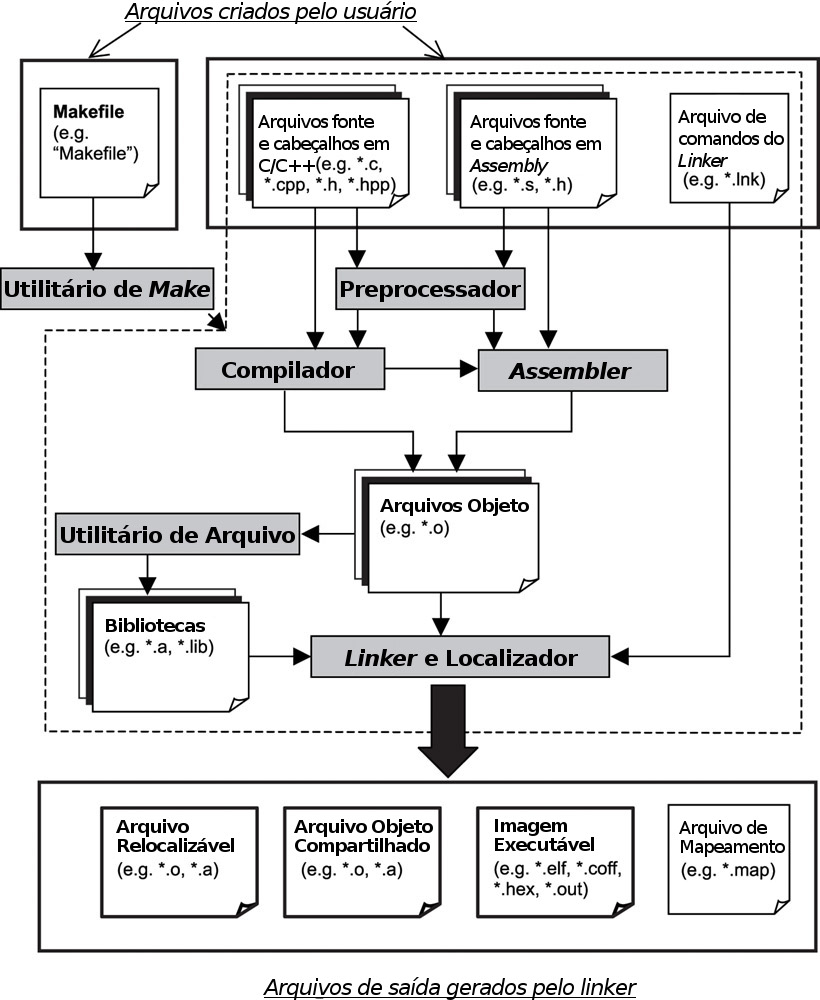
\includegraphics[scale=1]{dados/figuras/Linker.png}
%     \caption{Criando um arquivo de imagem para um sistema operacional alvo.\newline Fonte:\cite{Qing2003}}
%     \label{linker}
%\end{figure}

O \linker\ precisa combinar esses arquivos objetos e fundir as seções de diferentes arquivos em um segmento de programa. Esse processo cria uma única imagem executável para o sistema embarcado alvo. O desenvolvedor utiliza comandos de \linker\ (chamados de \textit{linker directives}) para controlar como o \linker\ combina essas seções e aloca seus segmentos no sistema alvo. As diretivas de \linker\ ficam contidas no arquivo de comando de \linker. O objetivo de criar esse arquivo de comando de \linker\ é para que o desenvolvedor de sistemas embarcados possa mapear a imagem executável para o \textit{hardware} alvo de forma precisa e eficiente. 

\begin{figure}[H]
    \scriptsize
     \centering
     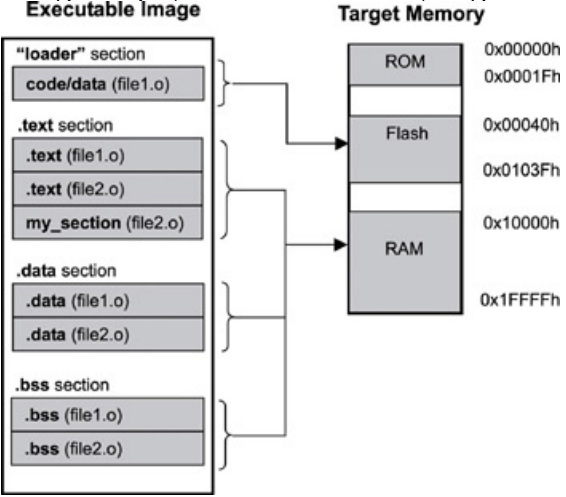
\includegraphics[scale=0.7]{dados/figuras/Linker4.png}
     \caption{Mapeando uma imagem executável em um sistema alvo.\newline Fonte:\cite{Qing2003}}
     \label{linker}
\end{figure}







\section {COMUNICAÇÃO CLIENTE-SERVIDOR}

Um programa cliente é um programa que funciona em um sistema computacional, que solicita e recebe um serviço de um programa servidor, que funciona em outro sistema final. Uma vez que o programa cliente é executado em um computador e o programa servidor, é executado em outro, aplicações cliente-servidor são, por definição, aplicações distribuídas. Os programas cliente e o servidor interagem enviando mensagens um para o outro, pela internet ou qualquer outra rede local ou remota. Neste nível de abstração, os roteadores, enlaces e outros componentes da internet funcionam como uma caixa-preta que transferem mensagens entre os componentes distribuídos, comunicantes, de uma aplicação \cite{Kurose2010}.

A comunicação cliente-servidor na internet é feita por meio de diversos protocolos de rede, cujo conjunto de protocolos é conhecido como pilha TCP/IP (\textit{Transmission Control Protocol/Internet Protocol}). Essa pilha é dividida em quatro camadas, em que cada camada é encarregada de realizar uma série de funções, concedendo um grupo de serviços bem definidos para o protocolo da camada superior. A \autoref{fig:PilhaTCP} ilustra a pilha TPC/IP e seus protocolos. 

\begin{figure}[H]
    \scriptsize
     \centering
     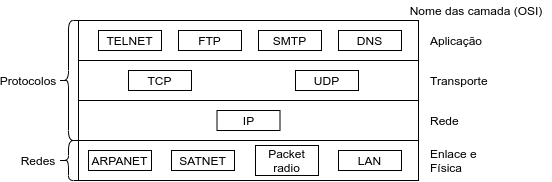
\includegraphics[scale=1]{dados/figuras/PilhaTCP-IP.png}
     \caption{Pilha TCP/IP e seus protocolos.\newline Fonte:\cite{tanenbaumRedes}}
     \label{fig:PilhaTCP}
\end{figure}

Essas camadas são denominadas:

\begin{itemize}
    \item Camada de aplicação: em que residem os protocolos de nível mais alto. Um protocolo da camada de aplicação é distribuído por diversos sistemas finais, sendo que a aplicação em um sistema usa o protocolo para trocar pacotes de informação com a aplicação em outro sistema.
    Exemplos de protocolos:
    \begin{itemize}
        \item HTTP (\textit{Hypertext transfer protocol}).
        \item SMTP (\textit{Simple Mail Transfer Protocol}). 
        \item FTP (\textit{File Transfer protocol}).
        \item DNS (\textit{Domain Name System}).
    \end{itemize}
    \item Camada transporte: em que reside os protocolos que fazem o transporte de dados da camada de aplicação, transportando mensagens entre os lados do cliente e do servidor de uma aplicação.
    Exemplos de protocolos:
    \begin{itemize}
        \item TCP (\textit{Transmission Control Protocol}).
        \item UDP (\textit{User Datagram Protocol}).
    \end{itemize}
    \item Camada de rede: camada que contém o protocolo responsável pela movimentação, de uma máquina para outra, de pacotes de camada de rede conhecidos como datagramas. Um protocolo da camada de transporte passa um segmento TCP ou UDP e um endereço de destino à camada de rede. A camada de rede prove o serviço de entrega do segmento à camada de transporte da máquina destinatária. O protocolo da camada de rede é chamado de IP (\textit{Internet Protocol}).
    \item Camada de enlace: é a camada que contém os protocolos que ficam responsáveis por enviar datagramas de um nó a outro, ou seja, faz o transporte do datagrama entre elementos da rede, como de uma máquina ao roteador, ou de roteador para roteador. Exemplos de protocolos:
    \begin{itemize}
        \item Arpanet.
        \item LAN (\textit{local area network}).
        \item WLAN (\textit{wireless local area network}).\newline
    \end{itemize}

\end{itemize}

Com a popularização da internet essa comunicação se tornou cada vez mais comum, atingindo bilhões de usuários no mundo todo. Assim a comunicação cliente servidor precisa ser segura. A segurança de redes se preocupa em garantir que pessoas mal-intencionadas não leiam ou modifiquem secretamente mensagens enviadas a outro destinatário. Ela também lida com meio de identificar se uma mensagem recebida é verdadeira e tem uma origem confiável \cite{tanenbaumRedes}.



\subsection{LWIP}
%Com a necessidade de se obter os binários dos códigos do novo firmware o sistema irá se utilizar da biblioteca amplamente conhecida e utilizada LWIP.
A Biblioteca LwIP é uma implementação da pilha TCP/IP, focada em ser pequena e portável, reduzindo a utilização de recursos como memória RAM e ainda tendo um TCP completo, se tornando adequada para sistemas embarcados. Foi originalmente desenvolvida por Adam Dunkels nos laboratórios da \textit{Computer and Networks Architectures} (CNA), no Instituto Sueco de Ciência da Computação (SICS) e agora é desenvolvida e mantida por uma rede mundial de desenvolvedores \cite{LWIP}.

Possui três \textit{Aplication Programing Interfaces} (APIs):
\begin{itemize}
\item RAW API (API básica): É a API nativa do LwIP, possui melhor desempenho e o menor tamanho de código, porém torna o desenvolvimento de aplicações mais complexo.
\item Netconn API: É uma API sequencial de alto nível que requer um sistema operacional de tempo real (RTOS). Habilita operações com múltiplas \textit{threads}.
\item BSD Sockets API: API de \textit{sockets} de Berkeley, desenvolvida em cima da API Netconn.
\end{itemize}

Essas API's implementam diversos protocolos de rede, incluindo:
\begin{itemize}
    \item HTTP permite a obtenção de recursos, tais como documentos HTML, imagens, scripts e outros tipos de arquivos.
    \item FTP para o envio e recebimento de arquivos.
    \item SMTP para o envio de mensagens de correio eletrônico através da internet.
    \item ICMP (\textit{Internet Control Message Protocol}) para manutenção e \textit{debugging} da rede.
    \item TCP com controle de congestionamento, estimativa de latência, recuperação e retransmissão rápida.
    \item IP incluindo o envio de pacotes para múltiplas interfaces de rede. \newline
    
 
    
\end{itemize} 

A seguir serão explanados com mais profundidade alguns dos protocolos implementados pela LwIP que serão utilizados neste trabalho.

\subsubsection{HYPERTEXT TRANSFER PROTOCOL (HTTP)}
Segundo \citeonline{Kurose2010}, o protocolo da camada de aplicação HTTP é implementado em dois programas, um programa cliente e outro servidor. Os dois são executados em sistemas finais diferentes, se comunicam entre eles por meio de uma troca de mensagens HTTP. O HTTP define a estrutura dessas mensagens assim como o modo como o cliente e o servidor as trocam. 

O HTTP define como clientes requisitam documentos aos servidores e como eles os transferem ao cliente. Ele utiliza o TCP como seu protocolo de transporte subjacente. O cliente HTTP primeiramente inicia uma conexão TCP com o servidor. Após essa conexão ser estabelecida, os processos da aplicação e do servidor acessam o TCP por meio de sua interface de sockets. No lado do cliente a interface de socket é uma porta entre o processo cliente e a conexão TCP. No lado do servidor, ela é uma porta entre o processo servidor  e a conexão TCP.

O cliente envia mensagens de requisição HTTP para sua interface de socket e recebe uma mensagem de resposta HTTP de sua interface de socket. De uma maneira parecida acontece do lado do servidor, onde ele recebe mensagens de requisição HTTP de sua interface de socket e envia mensagens respostas a sua interface. Assim a mensagem sai da camada de aplicação e passa para a camada de transporte. 

\subsubsection{TRANSMISSION CONTROL PROTOCOL (TCP)}

Segundo \citeonline{tanenbaumRedes}, O TCP foi projetado especificamente para oferecer um fluxo de bytes fim a fim confiável em uma inter-rede não-confiável. Uma inter-rede é diferente de uma única rede porque suas diversas partes podem ter topologias, larguras de banda, retardos, tamanhos de pacotes e outros parâmetros totalmente diferentes. O TCP foi projetado para se adaptar dinamicamente às propriedades da inter-rede e ser robusto diante de muitos categorias de falhas que podem ocorrer.

Cada máquina compatível com TCP tem uma entidade de transporte TCP, que pode ser um procedimento de biblioteca, um processo do usuário ou parte do núcleo. Em todos os casos, ele gerencia fluxos e interfaces TCP para a camada IP. Uma entidade TCP aceita fluxos de dados de usuários provenientes de processos locais, divide-os em partes de no máximo 64 kB e envia cada parte em um datagrama IP distinto. Quando os datagramas IP que contem dados TCP chegam a uma máquina, eles são enviados à entidade TCP, que restaura o fluxo de bytes originais.

A camada IP não oferece garantia que os datagramas serão entregues de forma apropriada, portanto, cabe ao TCP administrar os \textit{timers} e retransmiti-los sempre que necessário. Os datagramas também podem chegar fora de ordem, o TCP também terá que os reorganizar em mensagens na sequência correta. 

\subsection{MBED TLS}
A biblioteca Mbed TLS foi desenvolvida para se integrar facilmente a aplicações embarcadas existentes, e fornecer os blocos de construção para uma comunicação segura, criptografia e gerenciamento de chaves. Como o seu intuito é ser o mais flexível possível, permite que sejam integrados ao sistema somente as funcionalidades necessárias, diminuindo assim o tamanho total que a biblioteca ocuparia no sistema \cite{mbedtls}.

A \autoref{mbedtlsFig} ilustra como a biblioteca cria uma camada intermediária entre a aplicação final e a camada TCP/IP, chamada de TLS (\textit{Transport Layer Security}). A Mbed TLS pode ser usada para criar um servidor e cliente SSL (\textit{Secure Sockets Layer})/TLS, fornecendo uma estrutura para a configurar e se comunicar por meio de um canal de comunicação SSL/TLS. A camada TLS criada depende diretamente dos módulos de análise de certificado, criptografia simétrica ou assimétrica e \hash\ da biblioteca utilizada.

\begin{figure}[H]
    \scriptsize
     \centering
     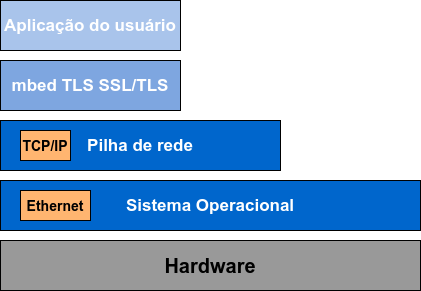
\includegraphics[scale=1]{dados/figuras/mbedtls.png}
     \caption{Pilha de comunicação.\newline Fonte:\cite{mbedtls}}
     \label{mbedtlsFig}
\end{figure}

A Mbed TLS provê a implementação da camada de segurança para a comunicação com o servidor, que pode evitar que uma versão maliciosa do software seja recebida de uma fonte não confiável. Também nos fornece peças de software contendo algoritmos criptográficos, que podem ser facilmente acoplados a qualquer aplicação. Como é o caso do algoritmo SHA-2 que ficará responsável por fazer a verificação da integridade dos arquivos baixados.

\subsubsection{TRANSPORT LAYER SECURITY (TLS)}

A \textit{Transport Layer Security} assim como seu precursor \textit{Secure Sockets Layer}, é um protocolo de segurança projetado para fornecer segurança na comunicação sobre uma rede de computadores.
Segundo \citeonline{TLSV12}, o protocolo TLS visa fornecer privacidade e integridade de dados entre aplicações que se comunicam. Quando uma rede está protegida por TLS, conexões entre um cliente e um servidor devem ter uma ou mais das seguintes propriedades:

\begin{itemize}
    \item A conexão é privada, pois, utilizada criptografia simétrica para criptografar os dados transmitidos. As chaves para essa criptografia são geradas exclusivamente para cada conexão e são baseadas em um segredo compartilhado que foi negociado no início da sessão (conhecido como \textit{Handshake Protocol}). No protocolo de \textit{Handshake}, o servidor e o cliente negociam qual algoritmo de criptografia e chaves criptográficas usar antes que o primeiro dado seja transmitido. Como a negociação ocorre somente no início da transmissão, qualquer invasor que intercepte a transmissão não poderá decifrar as mensagens, enviar dados e alterar os termos dessa negociação. Então a negociação de um segredo compartilhado é segura  e confiável.
    \item A conexão é confiável, pois cada mensagem transmitida inclui uma verificação de integridade de mensagem, utilizando um código de autenticação de mensagem, como uma \textit{hash} criptográfica, para evitar perda não detectada ou alteração dos dados durante a transmissão.
\end{itemize}

Uma vantagem do TLS é que ele é independente do protocolo da aplicação. No entanto, ele não especifica como os protocolos adicionam segurança ao TLS, as decisões sobre como iniciar o \textit{handshaking} e como interpretar os certificados de autenticação trocados são deixadas ao critério dos projetistas e desenvolvedores de protocolos executados sobre o TLS.

\subsubsection{FUNÇÃO HASH}

Segundo \citeonline{Kurose2010}, uma função \textit{hash} é um algoritmo que recebe uma entrada, $m$, e computa uma cadeia de bits de tamanho fixo $H(m)$ conhecida como \textit{hash}. Uma função de \textit{hash} criptográfica deve apresentar a seguinte propriedade:
no processamento, é impraticável encontrar duas mensagens diferentes $x$ e $y$ em que $H(x)=H(y)$.

A SHA-1 (Secure \textit{Hash} Algorithm) é um conjunto de funções \textit{hash} criptográficas projetadas pela NSA\cite{NSA}. Esse algoritmo, de forma resumida, se baseia em processar um resumo de mensagem de 160 bits por meio de um processo de quatro etapas, formado por uma etapa de enchimento(Adicionando 'uns' seguidos de 'zeros' suficientes, de maneira em que o comprimento da mensagem satisfaça determinados critérios), uma etapa de anexação (anexação de uma representação de alguns bits do comprimento da mensagem antes do enchimento), uma etapa de inicialização de um acumulador e uma etapa final iterativa, em que os blocos de palavras da mensagem são processados (misturados) em quatro rodadas de processamento. 

Comparando o \hash\ computado (a saída de execução do algoritmo) a um valor de \hash\ conhecido e esperado, pode-se determinar a integridade dos dados. Por exemplo, calcular o \hash\ de um arquivo baixado e comparar o resultado com um \hash\ conhecido, pode comprovar que o arquivo foi modificado ou adulterado.
SHA-2 é um conjunto de funções \hash\ criptográficas que contém mudanças significativas de seu antecessor. É composta por seis funções \hash\ com valores de \hash\ que são de 224, 256, 384 ou 512 bits: SHA-224, SHA-256, SHA-384, SHA-512, SHA-512/224, SHA-512/256.



%\section{CARTÃO SD}
\section{SISTEMAS DE ARQUIVO}
Segundo \citeonline{tanenbaumSO}, para resolver diversos problemas com o armazenamento de grandes quantidades de dados, a perda de dados após o fim da execução do processo que os criou e a necessidade de tornar esses dados independentes de quaisquer processos. Existe a necessidade da criação de uma estrutura de armazenamento de informações a longo prazo. Os três requisitos fundamentais para essa estrutura são:

\begin{itemize}
    \item Deve ser possivel armazenar um volume grande de informações.
    \item Os dados devem sobreviver ao término do processo que os estão utilizando.
    \item Vários processos devem ser capazes de acessar os dados concomitantemente.
\end{itemize}

Essa estrutura é chamada de arquivo, e é vastamente utilizada por diversos sistemas. Os arquivos são utilizados para armazenar dados em discos e outras mídias externas. Então os processos podem ler e escrever novos dados quando necessário. As informações armazenadas em arquivos devem ser persistentes, logo, não devem ser afetadas pela criação e pelo término do processo. Um arquivo só deve desaparecer quando o seu criador o apagar.

O modo como os arquivos são estruturados, nomeados, acessados, usados, protegidos e implementados são definidos geralmente pelo sistema operacional. A parte do sistema operacional responsável por esse gerenciamento é chamada de sistema de arquivos. Os arquivos podem, no caso de sistemas embarcados, ser gerenciados por API's que criam uma camada independente do sistema operacional e gerenciam os arquivos, como é o caso da biblioteca FatFs. 

Existem diversas formas de implementar um sistema de arquivo. Nessa implementação é necessário saber como os arquivos e seus diretórios são armazenados, como o espaço em disco é gerenciado e em como fazer tudo funcionar de modo eficiente e confiável. 
Um dos sistemas de arquivos padrões para o uso em memórias que são divididas em bloco é o FAT32. 
Um cartão SD é um dispositivo de memória não volátil criado pela SD Card Association \cite{SDCARD}, que possui sua memória dividida em blocos e que por padrão faz uso do sistema de arquivo FAT.




\subsection{SISTEMA DE ARQUIVO FAT}

Segundo \citeonline{tanenbaumSO}, o sistema de arquivo FAT (\textit{File Allocation Table}) é implementado por meio de uma alocação de memória encadeada usando uma tabela na memória. Nessa organização, o bloco de memória inteiro está disponível para dados. Além disso, o acesso aleatório é muito mais fácil. Mesmo que o encadeamento ainda tenha que ser seguido para encontrar determinado deslocamento dentro do arquivo, ele está inteiramente na memória. De modo que, pode ser seguido sem necessidade nenhuma de referenciar o disco.

A \autoref{FAT} ilustra como é a tabela, mostrando que o arquivo $A$ inicia-se no bloco 4 e segue o encadeamento até o seu fim, assim como o arquivo $B$ que se inicia no bloco 6. Ambos terminam com um marcador especial que no caso é o número -1.

\begin{figure}[H]
    \scriptsize
     \centering
     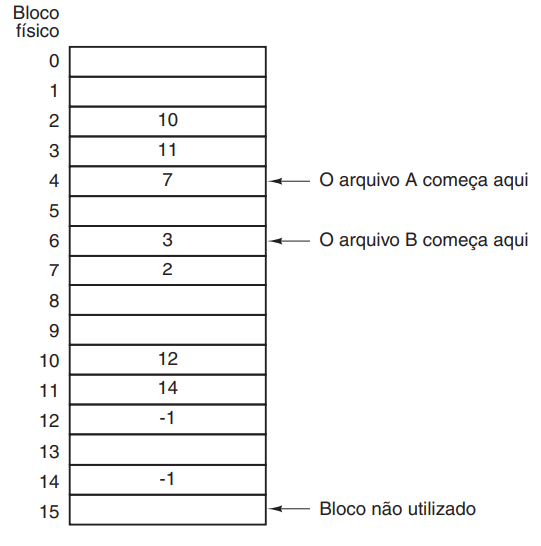
\includegraphics[scale=0.7]{dados/figuras/FAT.png}
     \caption{Alocação encadeada usando tabela de alocação de arquivo.\newline  Fonte:\cite{tanenbaumSO}}
     \label{FAT}
\end{figure}

A principal desvantagem deste método é que a tabela inteira precisa estar na memória o tempo todo. Com um disco de 20 GB e um tamanho de bloco de 1 KB, a tabela precisa de 20 milhões de entradas, uma para cada um dos 20 milhões de blocos do disco. Cada entrada tem de ter no mínimo 3 bytes para manter o endereço dos blocos. Para facilitar sua pesquisa, as entradas acabam ocupando 4 bytes. Assim, a tabela ocupará 60 MB ou 80 MB de memória principal o tempo todo, dependendo do sistema para ser otimizado para espaço ou para tempo.

Existe também o sistema de arquivo exFAT que é utilizado para mídias com capacidade de armazenamento maiores que 4 GB, que foi adotada como sistema de arquivo padrão para cartões de memória (SD card) maiores de 4 GB, pela SD Card Association \cite{SDCARD}.

\subsection{FATFS}

FatFs é um módulo genérico de um sistema de arquivo FAT/exFAT, para pequenos sistemas embarcados com recursos computacionais reduzidos. É escrito em conformidade com a ANSI C (C89) e é completamente separado da camada de entrada e saída do sistema, portanto, é independente da plataforma utilizada. É um \software\ livre de código aberto e proporciona a leitura, escrita, criação e remoção de arquivos, além do gerenciamento e navegação de diretórios. A \autoref{FatFS} ilustra como o módulo é independente da aplicação e da plataforma utilizada.

\begin{figure}[H]
    \scriptsize
     \centering
     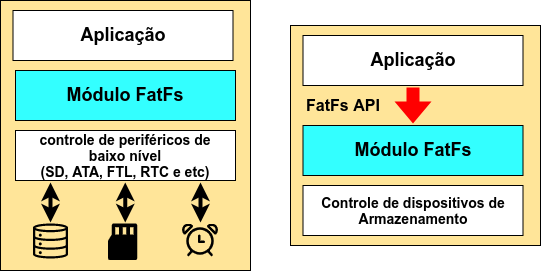
\includegraphics[scale=0.6]{dados/figuras/fatfs.png}
     \caption{Posição da biblioteca FatFs na aplicação.\newline  Fonte:\cite{FATFS}}
     \label{FatFS}
\end{figure}
A FatFs fornece várias funções do sistema de arquivos para a aplicação.
Assim pela aplicação é possível gerenciar os arquivos e diretórios, como é ilustrado da \autoref{FatFS2}. Umas das principais funções fornecidas pela FatFs para a aplicação são:

\begin{itemize}
    \item Acesso a arquivos.
    \begin{itemize}
        \item f\_open - Abre/Cria um arquivo.
        \item f\_close - Fecha um arquivo aberto.
        \item f\_read - Lê os dados de um arquivo.
        \item f\_write - Escreve dados em um arquivo.
    \end{itemize}
    \item Acesso a diretórios.
    \begin{itemize}
        \item f\_opendir - Abre um diretório.
        \item f\_closedir - Fecha um diretório aberto.
    \end{itemize}
    \item Gerenciamento de arquivos e diretórios.
    \begin{itemize}
        \item f\_stat - Verifica a existência de um arquivo ou diretório.
        \item f\_unlink - Remove um arquivo ou diretório. 
        \item f\_rename - Renomeia ou move um arquivo, ou diretório.
        \item f\_mkdir - Cria um diretório.
        \item f\_chdir - Muda o diretório atual.
    \end{itemize}
    \item Gerenciamento de volume e configurações do sistema.
    \begin{itemize}
        \item f\_mount - Registra ou remove registro da área de trabalho da partição.
        \item f\_mkfs - Cria uma partição FAT na unidade lógica.
        \item f\_fdisk - Cria uma partição na unidade física.
        \item f\_getfree - Obtém o espaço livre da partição.
    \end{itemize}
\end{itemize}

\begin{figure}[H]
    \scriptsize
     \centering
     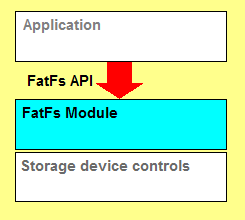
\includegraphics[scale=0.6]{dados/figuras/fatfs2.png}
     \caption{Manipulação da memória por meio da API da FatFs.\newline  Fonte:\cite{FATFS}}
     \label{FatFS2}
\end{figure}
%\section{SERVIDORES HTTP}

%É uma boa prática iniciar cada novo capítulo com um breve texto introdutório (tipicamente, dois ou três parágrafos) que deve deixar claro o quê será discutido no capítulo, bem como a organização do capítulo.
%Também servirá ao propósito de "amarrar"{} o conteúdo deste capítulo com o conteúdo do capítulo imediatamente anterior.


\section{TRABALHOS CORRELATOS}

Foram identificados três trabalhos correlatos.

%pode ter latencia de interrupção porem deve ser controlada

\begin{itemize}

    \item \textbf{Firmware over the air for automotive, Fotamotive}: Esse trabalho introduz uma solução para atualização de veículos com a ajuda de fabricantes de equipamentos altomotivos para reduzir custos com \textit{recalls} e assim aumentar a qualidade de seus produtos, facilitar as atualizações e controlar melhor a frota de veículos no mercado. Essa solução consiste em atualizar a unidade de controle do motor por meio de métodos OTA, sem a necessidade de uma conexão física com o veículo \cite{Odat2014}.

    \item \textbf{Firmware over the air for home cybersecurity in the Internet of Things}: Esse trabalho descreve a utilização de um método de atualização de \firmware\ para roteadores caseiros, utilizando sistemas de gerenciamento de rede e de suporte de operações de fornecedores de acesso à \textit{internet} \cite{Teng2017}.
    
    \item \textbf{Internet of Things: Over-the-Air (OTA) firmware update in Lightweight mesh network protocol for smart urban development}: Esse trabalho introduz um novo sistema de atualização de \firmware\ \textit{Over-The-Air} (OTA) baseado no protocolo de rede \textit{Lightweight mesh}, que prove descoberta de rotas, estabelecimento e um protocolo de malha de baixa potência \cite{Chandra2016}.

\end{itemize}

Como observado, todos os trabalhos correlatos tem um objetivo único e diferente para a aplicação de sua atualização OTA, enquanto esse trabalho tem como meta produzir um sistema que pode abranger diferentes aplicações.         % Revisão de Literatura
% METODOLOGIA

\chapter{SISTEMA DE ATUALIZAÇÃO DE FIRMWARE OVER-THE-AIR}
\label{chap:metodologia}
Nesse capitulo é retratado como será o funcionamento do sistema que será desenvolvido, mostrada uma visão geral do projeto, listada as funcionalidades de cada uma das partes do \textit{software}, explicando sua atividade, sua implementação, e as ferramentas utilizadas para o seu teste e os materiais utilizados. 

\section{VISÃO GERAL}
O \textit{software} que será desenvolvido nesse trabalho é dividido em duas partes, uma contendo o \bootloader, com o auxílio da biblioteca FatFs, que é um módulo genérico do sistema de arquivo FAT, realizará a comunicação com o cartão SD, que conterá o novo \firmware\ previamente recebido. Assim poderá substituir o \software\ anterior da aplicação por um novo. Essa parte do \software\ ficará armazenada em uma região da memória que dificilmente será reescrita, podendo ser reescrita somente com o auxílio de ferramentas de desenvolvimento como um JTAG e/ou \textit{debugger}, então é uma peça do programa que dificilmente será substituída. Será uma parte que não é portável para todas as plataformas, ficando a cargo do projetista fazer o porte para outras placas.

A outra parte desse trabalho será uma API, contendo as demais funções necessárias para a comunicação com o servidor, que enviará para o sistema o novo \firmware, por meio do uso da biblioteca LwIP, garantirá a segurança dessa conexão com a utilização de uma camada extra de proteção, com biblioteca Mbed TLS. Essa API irá conectar-se a um servidor em um intervalo de tempo determinado pelo projetista, em que verificará a disponibilidade de uma nova versão de \software. 

Após ser confirmada a existência de uma nova versão de \firmware, em um tempo determinado pelo projetista a API irá se comunicar novamente com o servidor com o intuito de fazer o \download\ dessa nova versão, e a armazenar em um endereço de memória predeterminado no cartão SD do sistema, para que então o \bootloader\ entre em ação após uma reinicialização do sistema.
A API será uma peça de \software\ que poderá ser substituída e atualizada em conjunto com as demais aplicações do sistema, como, as bibliotecas LwIP, Mbed TLS, o sistema operacional, entre outras peças de \software\ utilizadas pela aplicação. 

O sistema de atualização OTA utiliza-se de bibliotecas já conhecidas e vastamente utilizadas por desenvolvedores de sistemas embarcados. Para que assim projetos que necessitem fazer comunicação segura via rede, leitura e escrita de cartões SD, possam utilizar esse sistema de modo a poupar espaço na memória, visando a reutilização dessas bibliotecas. Portanto, o sistema pode ser amplamente utilizado por sistema de IoT. 
%Será utilizada o \textit{kit} de desenvolvimento STM32F746G \textit{Discovery}, onde será inicialmente desenvolvida a API, suas tarefas e o \textit{bootloader} que serão os principais componentes desse sistema.

Em caso de uma falha durante o processo de atualização OTA e o sistema não responda após a atualização, o sistema tem a habilidade de se recuperar. Como não haverá sobreescrita na área em que o \textit{firmware} está posicionado no cartão SD, uma simples reinicialização do sistema pode fazer com que o bootloader seja ativado novamente e refaça o processo de cópia da memória.

O sistema de atualização irá funcionar da seguinte forma, após a inicialização do sistema o \bootloader\ entra em ação e verifica a existência de um novo \firmware, no caso negativo ele inicia normalmente o \software\ principal da aplicação. No caso positivo, o \bootloader\ inicia o processo de substituição de \textit{firmware}, após a troca, o novo \software\ é iniciado. Durante a execução da aplicação principal do sistema e em um tempo determinado pelo projetista a API entra em contato com o servidor para verificar a disponibilidade de um \software\ novo, em caso positivo ela agenda um período para a atualização do \firmware, no caso negativo ele continua a execução da aplicação. 

Caso haja uma atualização quando o horário do agendamento chegar, a API irá conectar-se ao servidor e iniciar o processo de \download\ do \firmware\ novo e armazena-lo em uma área já predefinida do cartão SD para que o \bootloader\ possa o encontrar. Após o \download\ o sistema irá ser reiniciado e o \bootloader\ entrará em ação novamente. 
%De forma resumida o funcionamento do sistema pode ser visto na \autoref{Funcionamento}, 


%Com a  As tarefas serão produzidas a partir de b
%sistema possa conter intersecções com trechos de codigos utilizados em varios projetos que necessitam

%Adicionar diagrama de blocos!!!!

% A seguir será explicado parcialmente como funcionarão as funções das tarefas, do \textit{bootloader}, e do servidor HTTP.
%Cada capítulo deve conter uma pequena introdução (tipicamente, um ou dois parágrafos) que deve deixar claro o objetivo e o que será discutido no capítulo, bem como a organização do capítulo.

\section{\textit{BOOTLOADER}}
\label{sec:Bootloader}

A partir de um arquivo de \textit{linker}, a memória da plataforma será customizada com o intuito de abrigar os arquivos necessários para o \bootloader\ e protegê-lo de eventuais sobrescritas que podem vir a ocorrer. Esse arquivo de \textit{linker}, assim como o próprio \textit{bootloader}, será escrito somente para a plataforma STM32F7, visto que cada plataforma tem suas próprias características como, tamanho de memória e endereços diferentes para cada fabricante e/ou arquitetura.

No arquivo de \linker\ será especificada uma área especial na memória flash do sistema em que será abrigado o \bootloader\ e a biblioteca FatFs que fará parte do \bootloader. Também será responsável por fazer com que o \bootloader\ seja chamado no lugar da função \textit{main}. Assim podemos garantir que o \bootloader\ sempre entre em ação após a reinicialização do sistema embarcado.

%irá verificar o \textit{hash} da nova versão, verificando a integridade e origem do \textit{software},

O \textit{bootloader} será responsável em fazer a troca de cada versão de \textit{firmware} instalado no sistema embarcado. Sempre que o sistema for iniciado, o \textit{bootloader} será inicializado e fará a procura de um novo \textit{firmware} em um endereço de memória já predeterminado. Essa busca será possível pelo fato da biblioteca FatFs, que está implementada junto ao \bootloader, criar um sistema de arquivos no cartão SD do sistema alvo, assim o \bootloader\ pode acessar a memória do cartão sem a necessidade da a aplicação final ser inicializada.

Se a procura retornar com um resultado positivo para a existência de uma nova versão de \software, o \bootloader\ inicia o processo de atualização. Nesse processo o \bootloader\ substitui completamente o \software\ e demais bibliotecas e API's em áreas não protegidas na memória, pelo binário do \textit{firmware} presente no cartão SD. Esse processo será implementado com o uso da função memcpy, já conhecida e utilizada por diversos desenvolvedores, com o intuito de se deixar o código do \bootloader\ mais reutilizável. O funcionamento resumido do \textit{bootloader} pode ser observado na \autoref{fig:DiagBootloader}.

\begin{figure}[H]
    \scriptsize
     \centering
     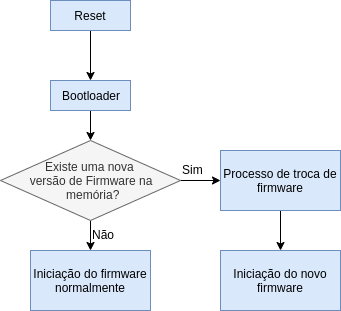
\includegraphics[scale=0.9]{dados/figuras/BootloaderDiag.png}
     \caption{Diagrama de funcionamento do \bootloader. \newline Fonte: autoria própria.}
     \label{fig:DiagBootloader}
\end{figure}
%Inserir seu texto aqui...

%\section{SERVIDOR HTTP}
%\label{sec:ServidorHTTP}

%A partir de um computador conectado à mesma rede que o sistema embarcado, haverá um servidor HTTP que ficará responsável por esperar requisições do dispositivo, para consultar a disponibilidade de uma versão atualizada do \textit{software}, e após a confirmação dessa nova versão, esse servidor irá enviar o \textit{firmware} para a plataforma embarcada.
%Inserir seu texto aqui...

\section{API DE ATUALIZAÇÃO OTA}
\label{sec:API}

A API de atualização OTA que será desenvolvida nesse trabalho tem o propósito de ser o mais portável possível, para assim, ser reutilizada por diversos projetos que necessitem da troca de seu \software. Com esse objetivo, serão utilizadas as bibliotecas já bem difundidas, a LwIP para a criação da pilha TCP/IP, a Mbed TLS para criar uma camada se segurança nessa pilha, e a FATFS para a criação de um sistema de arquivos FAT. Assim desenvolvedores podem se aproveitar do fato de que essas bibliotecas já estão em seus sistemas como padrão para utiliza-las em suas próprias funcionalidades. A \autoref{fig:DiagAPI} ilustra de forma resumida o funcionamento da API.

\begin{figure}[H]
    \scriptsize
     \centering
     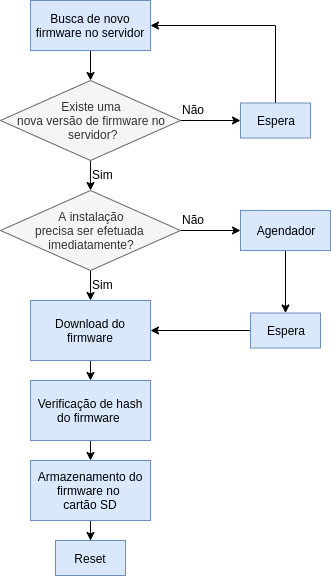
\includegraphics[scale=0.9]{dados/figuras/DiagAPI.png}
     \caption{Diagrama de funcionamento da API.\newline Fonte: autoria própria.}
     \label{fig:DiagAPI}
\end{figure}


A seguir será retratado como serão cada uma das funcionalidades necessárias na API.

\subsection{COMUNICAÇÃO COM O SERVIDOR}

Com o uso da biblioteca LwIP e Mbed TLS será criada uma pilha de comunicação no sistema alvo, que ficará responsável pela conexão segura com o servidor que fornecerá o novo firmware. Na implementação da pilha de comunicação, será utilizada a API BSD Sockets, pois, o intuito é deixar o sistema de atualização portável, e essa API fornece suporte a sistemas operacionais de tempo real.

Como a biblioteca Mbed TLS já foi desenvolvida para ser integrada facilmente a várias aplicações embarcadas, ela será utilizada para criar protocolos de segurança nessa comunicação com o servidor. Serão utilizados padrões SSL/TLS para ser criado um canal criptografado entre o servidor e o sistema alvo, para garantir que todos os dados transmitidos sejam sigilosos e seguros, e também algoritmos de criptografia para o \firmware\ que será enviado por meio dessa conexão.

%essa tarefa estará responsável por criar uma comunicação segura entre o \textit{hardware} e o servidor HTTP, a partir dessa comunicação será feito a verificação do sinal de disponibilidade de novo \textit{software} e \textit{download} do mesmo quando o sistema estiver ocioso. 

\subsection{VERIFICAÇÃO E AGENDAMENTO DE ATUALIZAÇÃO}

O desenvolvedor será responsável em decidir a frequência e/ou horário em que a API irá consultar o servidor para a verificação de uma nova versão de \textit{firmware}. A API evitará que em aplicações onde existam atividades críticas, elas sejam interrompidas para que a API possa fazer essa constatação, sabendo que a prioridade dessa ação deve ser a menor possível na aplicação.

Após a consulta, caso exista uma nova atualização disponível o desenvolvedor pode optar em a executar imediatamente, ou agendar para ser feita em outro horário, em que a aplicação esteja menos ocupada. Essa escolha pode ser programada desde o início do desenvolvimento do \firmware, ou a partir de um sinal durante a consulta por uma nova atualização. Assim caso haja a necessidade da troca de \software\ imediatamente, esse sinal pode avisar o agendador e já executar todo o processo de substituição de \firmware. 

\subsection{DOWNLOAD E ARMAZENAMENTO DO FIRMWARE}

Quando chegar no tempo esperado pelo agendador, a API iniciará novamente a comunicação com o servidor que contém o \textit{firmware} novo, dessa vez com o propósito de fazer \download\ da nova versão do \textit{software}. Com o propósito de aumentar a segurança da API o \textit{firmware} que se apresenta após a transferência ainda está criptografado, assim ele deve passar por uma descriptografia para então ser armazenado no cartão SD. Após essa descriptografia a API ainda irá verificar se o \textit{firmware} recebido pelo servidor está correto a partir da verificação de \textit{hash} criptográfica. 

A partir da utilização da biblioteca FatFs, será criado um sistema de arquivo FAT, que gerenciará a memória presente no cartão SD dentro da aplicação, e ele pode ser utilizado tanto pela aplicação final do sistema embarcado, quanto pela API. Esse sistema de arquivo será utilizado para que se possa identificar a posição na memória em que o \textit{firmware} novo será colocado após o seu \download, evitando que outros arquivos, pertencentes a aplicação final, sejam colocados nessa localização, e fazendo com que o \bootloader\ interprete de forma errada os arquivos gerando erros.


%maquina de estado para leitura do arquivo.
\section{MATERIAIS UTILIZADOS}

A API será escrita na linguagem C, o \textit{bootloader} em sua maioria em C também, e alguns trechos em \textit{assembly}, enquanto o \linker\ será escrito em comandos de \linker. A escrita desses códigos será feita com o uso do ambiente de desenvolvimento integrado Eclipse \cite{Eclipse}. O sistema de atualização OTA desenvolvido nesse trabalho será inicialmente desenvolvido para a plataforma STM32F746G-Discovery.

\subsection{PLATAFORMA STM32F746G-DISCOVERY}

O STM32F7 Discovery é um kit de desenvolvimento que permite ao usuário desenvolver e compartilhar aplicações com toda a série de microcontroladores STM32F7 baseados no processador ARM\textregistered  Cortex\textregistered-M7 core.
O kit discovery permite uma ampla diversidade de aplicações que podem se beneficiar de suporte a múltiplos sensores, áudio, tela gráfica, segurança, vídeos e conexões de alta velocidade \cite{STM32F7}.
A \autoref{STM32F7} ilustra o kit STM32F746NGH6-Discovery.

\begin{figure}[H]
    \scriptsize
     \centering
     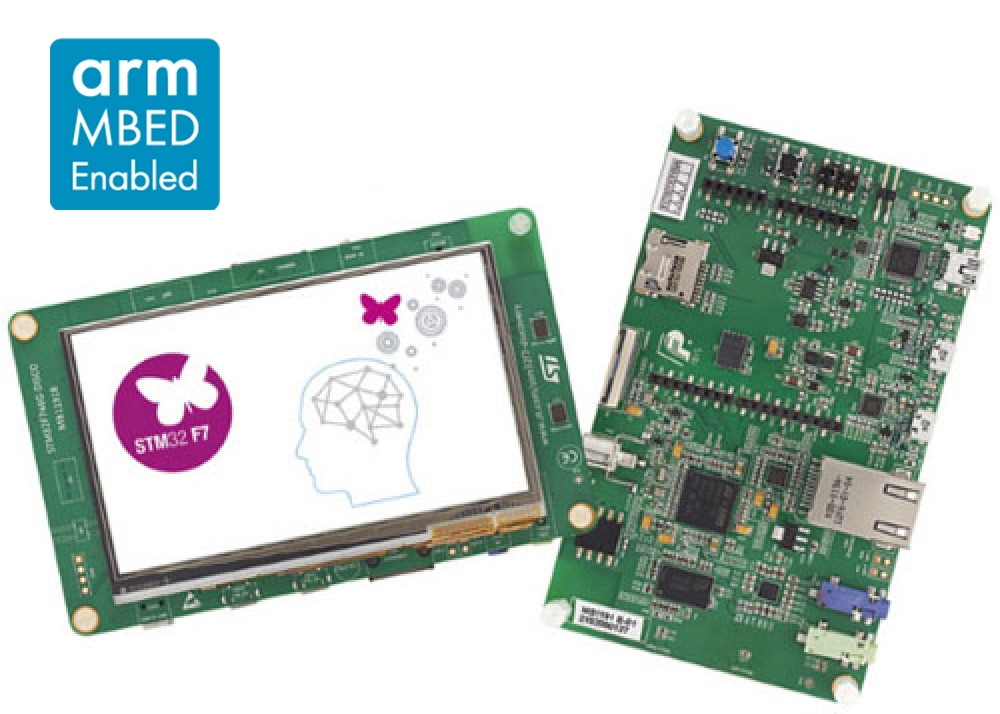
\includegraphics[scale=0.4]{dados/figuras/STM32F7.jpg}
     \caption{Kit de desenvolvimento STM32F746G-Discovery. \newline Fonte:\cite{STM32F7}.}
     \label{STM32F7}
\end{figure}

Algumas de suas principais características são:
\begin{itemize}
    \item Microcontrolador STM32F746NGH6 com 1 Mbytes de memória flash e 340 Kbytes de RAM, em um pacote BGA216.
    \item 128-Mbit de memória Quad-SPI Flash.
    \item 128-Mbit SDRAM (Com 64 Mbits Acessível).
    \item Conector para cartão microSD.
    \item Conector Ethernet em conformidade com a IEEE-802.3-2002
    \item Tela LCD de 4.3 polegadas, com resolução de 480x272 com \textit{touch-screen} capacitivo.
    
\end{itemize}                   % Metodologia
% RESULTADOS-------------------------------------------------------------------

%\chapter{ANÁLISE E DISCUSSÃO DOS RESULTADOS}
\chapter{CRONOGRAMA}
%Cada capítulo deve conter uma pequena introdução (tipicamente, um ou dois parágrafos) que deve deixar claro o objetivo e o que será discutido no capítulo, bem como a organização do capítulo.
\begin{enumerate}
    \item Estudo bibliográfico; 
    \item Desenvolvimento da proposta;
    \item Familiarização com plataforma;
    \item Projeto de \textit{bootloader} e tarefas;
    \item Entrega do TCC1;
    \item Desenvolvimento do \textit{bootloader};
    \item Criação do servidor HTTP;
    \item Implementação das tarefas;
    \item Testes de integração;
    \item Escrita da monografia e artigo científico.
 \end{enumerate}
 
    \begin{table}[h]
    \scriptsize
        \begin{tabular}{|c|c|c|c|c|c|c|c|c|c|c|}
\hline
\textbf{Atividade} & \textbf{08/19} & \textbf{09/19} & \textbf{10/19} & \textbf{11/19} & \textbf{12/19} & \textbf{01/20} & \textbf{02/20} & \textbf{03/20} & \textbf{04/20} & \textbf{05/20} \\ \hline
\textbf{1}         & X              & X              & X              & X              & X              & X              & X              & X              & X              & X              \\ \hline
\textbf{2}         & X              &                &                &                &                &                &                &                &                &                \\ \hline
\textbf{3}         & X              & X              & X              & X              &                &                &                &                &                &                \\ \hline
\textbf{4}         &                & X              & X              & X              & X              &                &                &                &                &                \\ \hline
\textbf{5}         &                &                &                &                & X              &                &                &                &                &                \\ \hline
\textbf{6}         &                &                &                &                & X              & X              & X              &                &                &                \\ \hline
\textbf{7}         &                &                &                &                &                & X              &                &                &                &                \\ \hline
\textbf{8}         &                &                &                &                &                & X              & X              & X              & X              &                \\ \hline
\textbf{9}         &                &                &                &                &                &                &                & X              & X              & X              \\ \hline
\textbf{10}        & X              & X              & X              & X              & X              & X              & X              & X              & X              & X              \\ \hline
\end{tabular}
\end{table}

                    % Resultados
%% ORIENTAÇÕES GERAIS------------------------------------------------------------

\chapter{UTILIZANDO O SISTEMA}
Com o intuito de fazer a ferramenta criada neste projeto ser facilmente utilizada por diversos desenvolvedores esse capitulo foi criado para facilitar o entendimento de como utilizar o sistema de atualização OTA proposto. Destacando como portar e utilizar o bootloader e toda a API do firmware OTA. Para a utilização de ambos os firmwares desenvolvidos neste trabalho é sempre necessário que as bibliotecas que são utilizadas por eles já estejam incluidas no projeto. Para o bootloader, é necessário somente a biblioteca FATFS, enquanto para o OTA são necessárias as bibliotecas FATFS, LWIP e MBED TLS.

\section{PORTANDO O BOOTLOADER}
Para se utilizar o bootloader proposto em outros sistemas embarcados da familia STM32 deve-se primeiramente observar a organização da memória FLASH do sistema microcontrolado que se deseja portar o bootloader. Como podemos observar na \autoref{STM32F7_FLASH} a memória FLASH do microcontrolador STM32F746NGH6 possui oito setores de memória com tamanhos distintos, para esse trabalho foi selecionado o primeiro setor de memória para abrigar o bootloader.

\begin{table}[H]
    \scriptsize
    \centering
    \begin{tabular}{|c|c|c|}

    \hline
    Nome    & Endereço do bloco         & Tamanho do setor \\ \hline
    Setor 0 & 0x0800 0000 - 0x0800 7FFF & 32 Kbytes        \\ \hline
    Setor 1 & 0x0800 8000 - 0x0800 FFFF & 32 Kbytes        \\ \hline
    Setor 2 & 0x0801 0000 - 0x0801 7FFF & 32 Kbytes        \\ \hline
    Setor 3 & 0x0801 8000 - 0x0801 FFFF & 32 Kbytes        \\ \hline
    Setor 4 & 0x0802 0000 - 0x0803 FFFF & 128 Kbytes       \\ \hline
    Setor 5 & 0x0804 0000 - 0x0807 FFFF & 256 Kbytes       \\ \hline
    Setor 6 & 0x0808 0000 - 0x080B FFFF & 256 Kbytes       \\ \hline
    Setor 7 & 0x080C 0000 - 0x080F FFFF & 256 Kbytes       \\ \hline
    \end{tabular}
    \caption{Organização do bloco de memória FLASH do microcontrolador STM32F746NGH6. \newline Adaptado de:\cite{STM32F7}.}
    \label{STM32F7_FLASH}
    \end{table}


Para isso foi necessário modificar no arquivo de linker o tamanho máximo da memória utilizável para evitar que os dados do bootloader ultrapassem o tamanho que determinamos para ele. Assim no arquivo de linker foi modificado de forma que o tamanho máximo da memória seja de 32Kbytes e iniciada no setor 0. Com isso a configuração de memória do bootloader para o microcontrolador utilizado neste trabalho ficou da seguinte forma:

\begin{lstlisting}
/* Specify the memory areas */
MEMORY
{
RAM (xrw)      : ORIGIN = 0x20000000, LENGTH = 320K
FLASH (rx)      : ORIGIN = 0x8000000, LENGTH = 32K
}
\end{lstlisting}

Como cada microcontrolador tem sua configuração de memória o desenvolvedor deve observar a configuração do sistema alvo e colocar sempre o bootloader no setor 0 de seu microcontrolador.

Feita a modificação no arquivo de linker o desenvolvedor iniciará a alteração do arquivo bootloader.h que contem algumas definições dependentes do seu microcontrolador. Neste arquivo as definições que precisam ser alteradas são:
\begin{itemize}
    \item FIRMWARE\_VERSION\_ADDRESS: Esta definição mostra ao bootloader a posição na memória FLASH em que se deve armazenar a versão atual da aplicação presente na placa e deve ser sempre os quatro últimos bytes da memória, e deve sempre ser o mesmo configurado na API de atualização OTA. No caso do microcontrolador deste trabalho foi utilizada a posição: 0x080FFFFC.
    \item FIRMWARE\_PATH: Esta definição mostra qual o caminho do arquivo em que se encontra o novo firmware que foi baixado pela API OTA, deve ser sempre igual ao que será definido na API.
    \item FIRMWARE\_NEW\_VERSION\_PATH: Esta definição mostra qual o caminho do arquivo em que se encontra a versão do novo firmware que foi baixado pela API OTA, deve ser sempre igual ao que será definido na API.
    \item APP\_START\_ADDRESS: Esta definição mostra ao bootloader a posição na memória FLASH em que se deve armazenar o inicio da aplicação que será trocada sendo sempre o inicio do setor 1. No caso do microcontrolador deste trabalho foi utilizada a posição: 0x08008000.
   
\end{itemize}

Com essas alterações já é possível utilizar o bootloader em sistemas embarcados que utilizam microcontroladores da família STM32, restando agora a configuração da aplicação que será utilizada em conjunto com o bootloader e a configuração da API de atualização OTA.

\section{CONFIGURAÇÃO DA API OTA}
Assim como no bootloader, a aplicação também precisa ter seu arquivo de linker modificado para evitar sobrescritas no espaço reservado para o bootloader e reservar o espaço necessário para a variável de versão. Com isso o desenvolvedor deve novamente observar a \autoref{STM32F7_FLASH} e verificar qual posição de memória se inicia sua aplicação e o tamanho total dela deve ser obtido com a seguinte formula:

\begin{equation}
    Tamanho\ da\ aplicacao = Final\ da\ FLASH - inicio\ do\ setor\ 1\ da\ FLASH - 4\ bytes 
    \label{eq:calculo_flash}
\end{equation}


Utilizando a formula para o microcontrolador STM32F746NGH6 temos que o inicio do setor 1 de memória é 0x08008000 e o fim do ultimo setor de memória é 0x080FFFFF, assim podemos obter os valores de de inicio e tamanho da aplicação e assim configurar o arquivo de linker da aplicação da seguinte forma:



\begin{lstlisting}
/* Specify the memory areas */
MEMORY
{
RAM (xrw)      : ORIGIN = 0x20000000, LENGTH = 320K
FLASH (rx)      : ORIGIN = 0x08008000, LENGTH = 0xF7FFB
}
\end{lstlisting}

Feitas as alterações necessárias no arquivo de linker o desenvolvedor tem que alterar algumas definições no arquivo ota\_server.h com o intuito de adequar a API de atualização OTA para a sua aplicação. Neste arquivo as definições que precisam ser alteradas são:

\begin{itemize}
    \item FIRMWARE\_VERSION\_ADDRESS: Esta definição mostra a aplicação a posição na memória FLASH em que se deve armazenar a versão atual da aplicação presente na placa e deve ser sempre os quatro últimos bytes da memória, e deve sempre ser o mesmo configurado no bootloader. No caso do microcontrolador deste trabalho foi utilizada a posição: 0x080FFFFC.
    \item FIRMWARE\_PATH: Esta definição mostra qual o caminho do arquivo em que de deve armazenar o novo firmware que deverá ser baixado pela API OTA, deve ser sempre igual ao que será definido no bootloader.
    \item FIRMWARE\_NEW\_VERSION\_PATH: Esta definição mostra qual o caminho do arquivo em que se deve armazenar a versão do novo firmware que será baixado pela API OTA, deve ser sempre igual ao que será definido no bootloader.
    \item BOOTLOADER\_START\_ADDRESS: Esta definição mostra a aplicação a posição na memória FLASH em que está armazenado o inicio do bootloader sendo sempre o inicio do setor 0. No caso do microcontrolador deste trabalho foi utilizada a posição: 0x08000000.
    \item FIRMWARE\_NEW\_VERSION\_HASH\_PATH: Esta definição mostra qual o caminho do arquivo em que de deve armazenar o hash do novo firmware para que se compare com o hash gerado pelo firmware baixado, assim fazendo um teste para verificar se o firmware baixado é integro.
    \item AUTH\_SERVER: Esta definição mostra qual deve ser o endereço do servidor em que se deve obter os arquivos necessários para a atualização de firmware, então deve ser personalizada para cada aplicação.
    \item AUTH\_PORT: Esta definição mostra qual deve ser a porta que se deve conectar no servidor, como estamos utilizando uma camada de TLS esta porta deve ser a 443.
    \item AUTH\_REQUEST\_VERSION: Esta definição mostra qual a requisição HTTP do arquivo contendo o número da nova versão que deverá ser baixada pela API.
    \item AUTH\_REQUEST\_FIRMWARE: Esta definição mostra qual a requisição HTTP do firmware da nova versão que deverá ser baixada pela API.
    \item AUTH\_REQUEST\_HASH: Esta definição mostra qual a requisição HTTP do arquivo contendo o hash da nova versão que deverá ser baixada pela API.
    \item SSL\_CA\_PEM: Esta definição mostra o certificado SSL utilizado na comunicação com o servidor.
\end{itemize}

Com essas definições corretamente configuradas pode-se utilizar facilmente a API de atualização OTA proposta neste trabalho ficando a cargo do desenvolvedor somente programar em sua aplicação o algoritmos que determina quando a função que inicia a atualização é chamada para que o processo de atualização OTA proposto neste trabalho se encarregue de fazer todo o processo de forma autónoma. 
















\begin{comment}
% SOBRE AS ILUSTRAÇÕES----------------------------------------------------------
\chapter{SOBRE AS ILUSTRAÇÕES}
\label{chap:apSobreIlust}

A seguir exemplifica-se como inserir ilustrações no corpo do trabalho. As ilustrações serão indexadas automaticamente em suas respectivas listas. A numeração sequencial de figuras, tabelas e equações também ocorre de modo automático.

Referências cruzadas são obtidas através dos comandos \verb|\label{}| e \verb|\ref{}|. Sendo assim, não é necessário por exemplo, saber que o número de certo capítulo é \ref{chap:fundamentacaoTeorica} para colocar o seu número no texto. Outra forma que pode ser utilizada é esta: \autoref{chap:fundamentacaoTeorica}, facilitando a inserção, remoção e manejo de elementos numerados no texto sem a necessidade de renumerar todos esses elementos.

% FIGURAS-----------------------------------------------------------------------
\chapter{FIGURAS}
\label{chap:figuras}

Exemplo de como inserir uma figura. A \autoref{fig:figura-exemplo1} aparece automaticamente na lista de figuras. Para saber mais sobre o uso de imagens no \LaTeX{} consulte literatura especializada \cite{Goossens2007}.

Os arquivos das figuras devem ser armazenados no diretório de "/dados".

\begin{figure}[!htb]
    \centering
    \caption{Exemplo de Figura}
    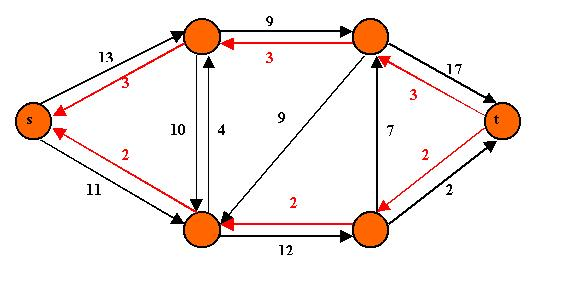
\includegraphics[width=0.5\textwidth]{./dados/figuras/figura1}
    \fonte{\citeonline{IRL2014}}
    \label{fig:figura-exemplo1}
\end{figure}

% QUADROS E TABELAS---------------------------------------------------------------
\chapter{QUADROS E TABELAS}
\label{chap:tabelas}

Exemplo de como inserir o \autoref{qua:quadro-exemplo1} e a \autoref{tab:tabela-exemplo1}. Ambos aparecem automaticamente nas suas respectivas listas. Para saber mais informações sobre a construção de tabelas no \LaTeX{} consulte literatura especializada \cite{Mittelbach2004}.

Ambos os elementos (Quadros e Tabelas) devem ser criados em arquivos separados para facilitar manutenção e armazenados no diretório de "/dados".

\begin{quadro}[!htb]
    \centering
    \caption{Exemplo de Quadro.\label{qua:quadro-exemplo1}}
    \begin{tabular}{|p{7cm}|p{7cm}|}
        \hline
        \textbf{BD Relacionais} & \textbf{BD Orientados a Objetos} \\
        \hline
        Os dados são passivos, ou seja, certas operações limitadas podem ser automaticamente acionadas quando os dados são usados. Os dados são ativos, ou seja, as solicitações fazem com que os objetos executem seus métodos. & Os processos que usam dados mudam constantemente. \\
        \hline
    \end{tabular}
    \fonte{\citeonline{Barbosa2004}}
\end{quadro}


A diferença entre quadro e tabela está no fato que um quadro é formado por linhas horizontais e verticais. Deve ser utilizado quando o conteúdo é majoritariamente não-numérico. O número do quadro e o título vem acima do quadro, e a fonte, deve vir abaixo. E Uma tabela é formada apenas por linhas verticais. Deve ser utilizada quando o conteúdo é majoritariamente numérico. O número da tabela e o título vem acima da tabela, e a fonte, deve vir abaixo, tal como no quadro.

\begin{table}[!htb]
    \centering
    \caption[Resultado dos testes]{Resultado dos testes.
    \label{tab:tabela-exemplo1}}
    \begin{tabular}{rrrrr}
        \toprule
            & Valores 1 & Valores 2 & Valores 3 & Valores 4 \\
        \midrule
            Caso 1 & 0,86 & 0,77 & 0,81 & 163 \\
            Caso 2 & 0,19 & 0,74 & 0,25 & 180 \\
            Caso 3 & 1,00 & 1,00 & 1,00 & 170 \\
        \bottomrule
    \end{tabular}
    \fonte{\citeonline{Barbosa2004}}
\end{table}


% EQUAÇÕES-----------------------------------------------------------------------
\chapter{EQUAÇÕES}
\label{chap:equacoes}

Exemplo de como inserir a \autoref{eq:equacao-exemplo1} e a Eq. \ref{eq:equacao-exemplo2} no corpo do texto \footnote{Deve-se atentar ao fato de a formatação das equações ficar muito boa esteticamente.}. Observe que foram utilizadas duas formas distintas para referenciar as equações.

\begin{equation}
    X(s) = \int\limits_{t = -\infty}^{\infty} x(t) \, \text{e}^{-st} \, dt
    \label{eq:equacao-exemplo1}
\end{equation}

\begin{equation}
    F(u, v) = \sum_{m = 0}^{M - 1} \sum_{n = 0}^{N - 1} f(m, n) \exp \left[ -j 2 \pi \left( \frac{u m}{M} + \frac{v n}{N} \right) \right]
    \label{eq:equacao-exemplo2}
\end{equation}

% ALGORITMOS-----------------------------------------------------------------------
\chapter{ALGORITMOS}
\label{chap:algoritmos}

Exemplo de como inserir um algoritmo. Para inserção de algoritmos utiliza-se o pacote {\ttfamily algorithm2e} que já está devidamente configurado dentro do template.

Os algoritmos devem ser criados em arquivos separados para facilitar manutenção e armazenados no diretório de "/dados".\\
\\

\begin{algorithm}
    \caption{Exemplo de Algoritmo}
    \KwIn{o número $n$ de vértices a remover, grafo original $G(V, E)$}
    \KwOut{grafo reduzido $G'(V,E)$}
    $removidos \leftarrow 0$ \\
    \While {removidos $<$ n } {
        $v \leftarrow$ Random$(1, ..., k) \in V$ \\
            \For {$u \in adjacentes(v)$} {
                remove aresta (u, v)\\
                $removidos \leftarrow removidos + 1$\\
            }
            \If {há  componentes desconectados} {
                remove os componentes desconectados\\
            }
        }
\end{algorithm}


% SOBRE AS LISTAS--------------------------------------------------------------------
\chapter{SOBRE AS LISTAS}
\label{chap:apSobreLista}

Para construir listas de "\textit{bullets}"{} ou listas enumeradas, inclusive listas aninhadas, é utilizado o pacote \verb|paralist|.

Exemplo de duas listas não numeradas aninhadas, utilizando o comando \verb|\itemize|. Observe a indentação, bem como a mudança automática do tipo de "\textit{bullet}"{} nas listas aninhadas.

\begin{itemize}
    \item item não numerado 1
    \item item não numerado 2
    \begin{itemize}
        \item subitem não numerado 1
        \item subitem não numerado 2
        \item subitem não numerado 3
    \end{itemize}
    \item item não numerado 3
\end{itemize}

Exemplo de duas listas numeradas aninhadas, utilizando o comando \verb|\enumerate|. Observe a numeração progressiva e indentação das listas aninhadas.

\begin{enumerate}
    \item item numerado 1
    \item item numerado 2
    \begin{enumerate}
        \item subitem numerado 1
        \item subitem numerado 2
        \item subitem numerado 3
    \end{enumerate}
    \item item numerado 3
\end{enumerate}

% SOBRE AS CITAÇÕES E CHAMADAS DE REFERÊNCAS----------------------------------------------
\chapter{SOBRE AS CITAÇÕES E CHAMADAS DE REFERÊNCAS}
\label{chap:apSobreCita}

Citações são trechos de texto ou informações obtidas de materiais consultadss quando da elaboração do trabalho. São utilizadas no texto com o propósito de esclarecer, completar e embasar as ideias do autor. Todas as publicações consultadas e utilizadas (por meio de citações) devem ser listadas, obrigatoriamente, nas referências bibliográficas, para preservar os direitos autorais. São classificadas em citações indiretas e diretas.

% CITAÇÕES INDIRETAS-----------------------------------------------------------------------
\chapter{CITAÇÕES INDIRETAS}
\label{chap:citacoesLivres}

É a transcrição, com suas próprias palavras, das idéias de um autor, mantendo-se o sentido original. A citação indireta é a maneira que o pesquisador tem de ler, compreender e gerar conhecimento a partir do conhecimento de outros autores. Quanto à chamada da referência, ela pode ser feita de duas maneiras distintas, conforme o nome do(s) autor(es) façam parte do seu texto ou não. Exemplo de chamada fazendo parte do texto:\\
\\Enquanto \citeonline{Maturana2003} defendem uma epistemologia baseada na biologia. Para os autores, é necessário rever \ldots.\\

A chamada de referência foi feita com o comando \verb|\citeonline{chave}|, que produzirá a formatação correta.

A segunda forma de fazer uma chamada de referência deve ser utilizada quando se quer evitar uma interrupção na sequência do texto, o que poderia, eventualmente, prejudicar a leitura. Assim, a citação é feita e imediatamente após a obra referenciada deve ser colocada entre parênteses. Porém, neste caso específico, o nome do autor deve vir em caixa alta, seguido do ano da publicação. Exemplo de chamada não fazendo parte do texto:\\
\\Há defensores da epistemologia baseada na biologia que argumentam em favor da necessidade de \ldots \cite{Maturana2003}.\\

Nesse caso a chamada de referência deve ser feita com o comando \verb|\cite{chave}|, que produzirá a formatação correta.

% CITAÇÕES DIRETAS-----------------------------------------------------------------------
\chapter{CITAÇÕES DIRETAS}
\label{chap:citacoesLiterais}

É a transcrição ou cópia de um parágrafo, de uma frase, de parte dela ou de uma expressão, usando exatamente as mesmas palavras adotadas pelo autor do trabalho consultado.

Quanto à chamada da referência, ela pode ser feita de qualquer das duas maneiras já mencionadas nas citações indiretas, conforme o nome do(s) autor(es) façam parte do texto ou não. Há duas maneiras distintas de se fazer uma citação direta, conforme o trecho citado seja longo ou curto.

Quando o trecho citado é longo (4 ou mais linhas) deve-se usar um parágrafo específico para a citação, na forma de um texto recuado (4 cm da margem esquerda), com tamanho de letra menor e espaçamento entrelinhas simples. Exemplo de citação longa:
\\\begin{citacao}
    Desse modo, opera-se uma ruptura decisiva entre a reflexividade filosófica, isto é a possibilidade do sujeito de pensar e de refletir, e a objetividade científica. Encontramo-nos num ponto em que o conhecimento científico está sem consciência. Sem consciência moral, sem consciência reflexiva e também subjetiva. Cada vez mais o desenvolvimento extraordinário do conhecimento científico vai tornar menos praticável a própria possibilidade de reflexão do sujeito sobre a sua pesquisa \cite[p.~28]{Silva2000}.
\end{citacao}

Para fazer a citação longa deve-se utilizar os seguintes comandos:
\begin{verbatim}
\begin{citacao}
<texto da citacao>
\end{citacao}
\end{verbatim}

No exemplo acima, para a chamada da referência o comando \verb|\cite[p.~28]{Silva2000}| foi utilizado, visto que os nomes dos autores não são parte do trecho citado. É necessário também indicar o número da página da obra citada que contém o trecho citado.

Quando o trecho citado é curto (3 ou menos linhas) ele deve inserido diretamente no texto entre aspas. Exemplos de citação curta:\\
\\A epistemologia baseada na biologia parte do princípio de que "assumo que não posso fazer referência a entidades independentes de mim para construir meu explicar" \cite[p.~35]{Maturana2003}.\\
\\A epistemologia baseada na biologia de \citeonline[p.~35]{Maturana2003} parte do princípio de que "assumo que não posso fazer referência a entidades independentes de mim para construir meu explicar".

% DETALHES SOBRE AS CHAMADAS DE REFERÊNCIAS---------------------------------------------------------
\chapter{DETALHES SOBRE AS CHAMADAS DE REFERÊNCIAS}
\label{chap:referUtilizadas}

Outros exemplos de comandos para as chamadas de referências e o resultado produzido por estes:\\
\\\citeonline{Maturana2003} \ \ \  \verb|\citeonline{Maturana2003}|\\
\citeonline{Barbosa2004} \ \ \   \verb|\citeonline{Barbosa2004}|\\
\cite[p.~28]{Silva2000} \ \ \  \verb|\cite[p.~28]{Silva2000}|\\
\citeonline[p.~33]{Silva2000} \ \ \   \verb|\citeonline[p.~33]{v}|\\
\cite[p.~35]{Maturana2003} \ \ \   \verb|\cite[p.~35]{Maturana2003}|\\
\citeonline[p.~35]{Maturana2003} \ \ \   \verb|\citeonline[p.~35]{Maturana2003}|\\
\cite{Barbosa2004,Maturana2003} \ \ \   \verb|\cite{Barbosa2004,Maturana2003}|\\

% SOBRE AS REFERÊNCIAS BIBLIOGRÁFICAS-------------------------------------------------------
\chapter{SOBRE AS REFERÊNCIAS BIBLIOGRÁFICAS}
\label{chap:apSobreRefer}

A bibliografia é feita no padrão \textsc{Bib}\TeX{}. As referências são colocadas em um arquivo separado. Neste template as referências são armazenadas no arquivo "base-referencias.bib".

Existem diversas categorias documentos e materiais componentes da bibliografia. A classe abn\TeX{} define as seguintes categorias (entradas):

\begin{verbatim}
@book
@inbook
@article
@phdthesis
@mastersthesis
@monography
@techreport
@manual
@proceedings
@inproceedings
@journalpart
@booklet
@patent
@unpublished
@misc
\end{verbatim}

Cada categoria (entrada) é formatada pelo pacote \citeonline{abnTeX22014d} de uma forma específica. Algumas entradas foram introduzidas especificamente para atender à norma \citeonline{NBR6023:2002}, são elas: \verb|@monography|, \verb|@journalpart|,\verb|@patent|. As demais entradas são padrão \textsc{Bib}\TeX{}. Para maiores detalhes, refira-se a \citeonline{abnTeX22014d}, \citeonline{abnTeX22014b}, \citeonline{abnTeX22014c}.

% NOTAS DE RODAPÉ--------------------------------------------------------------------------
\chapter{NOTAS DE RODAPÉ}
\label{chap:notasRodape}

As notas de rodapé pode ser classificadas em duas categorias: notas explicativas\footnote{é o tipo mais comum de notas que destacam, explicam e/ou complementam o que foi dito no corpo do texto, como esta nota de rodapé, por exemplo.} e notas de referências. A notas de referências, como o próprio nome ja indica, são utilizadas para colocar referências e/ou chamadas de referências sob certas condições.


\end{comment}                   % Capítulo com Orientações de uso do Template
%% CONCLUSÃO--------------------------------------------------------------------

\chapter{CONCLUSÃO}
\label{chap:conclusao}
O trabalho conseguiu alcançar o objetivo especifico de criar um sistema de atualização de firmware Over-The-Air utilizando as bibliotecas FatFs, MBED TLS e LWIP. Todos os objetivos específicos também foram atingidos visto que foi desenvolvido um bootloader que utiliza o sistema de aquivo FAT, foi implementada uma API que faz a comunicação com o servidor e armazena arquivos no cartão SD e assim foi comprovado o funcionamento do sistema na plataforma embarcada STM32F746NGH6-DISCOVERY.

Concluindo o trabalho foi possivel observar que o bootloader desenvolvido é muito mais portável que inicialmente se pensava. Como o processo de troca de firmware foi desenvolvido utilizando o HAL da STM foi possível fazer com que o bootloader funcione para toda a linha de microcontroladores da familia STM32 que possuam a biblioteca FatFS e acesso a um cartão SD. Alem de ser um bootloader robusto que consegue se recuperar em caso de falhas como quedas de energia durante o processo de troca de firmware.

A API que faz a busca dos arquivos no servidor HTTP e os armazena no cartao SD se mostrou perfeitamente funcional, conseguindo fazer a comparação de versões e a verificação de integridade do firmware baixado a partir de um hash baixado, deixando o sistema muito mais seguro contra falhas, além de conseguir fazer com que todo o sistema seja des-inicializado para fazer com que o bootloader seja executado em sua sequencia.

A implementação do sistema de atualização implementado na plataforma embarcada STM32F746NGH6 se mostrou efetuada com sucesso, conseguindo mostrar como diferentes firmwares puderam ser trocados de forma rápida, eficiente e dando ao usuário sinalizações que mostravam cada etapa do sistema.

Um dos revezes deste trabalho foi o fato que o sistema de atualização ocupa um espaço consideravel na memória flash dos microcontroladores, fazendo com que o sistema não funcione em hardwares com pouca memória, assim diminuindo a usabilidade do sistema, mas ainda é um ferramenta muito util e poderosa para sistemas mais robustos. Fazendo que que se abra a possibilidade de trabalhos futuros que possam melhorar ainda mais o sistema criado.
\section{TRABALHOS FUTUROS}
\label{sec:trabalhosFuturos}

Com o intuito de se tornar ainda mais robusto e ocupar uma quantidade de memória menor, este capitulo aborda algumas propostas de melhoria do sistema que podem ser feitas em trabalhos futuros. Essa proposta faz com que o sistema seja mais atrativo para ser utilizado em sistemas com uma quantidade menor de memória.

Uma proposta consiste em utilizar todas as ferramentas já utilizadas no bootloader no próprio firmware em será atualizado. O firmware pode a partir de ponteiros de função utilizar as funções presentes na biblioteca do FatFS e do HAL que já estão implementadas no bootloader em sua aplicação, não sendo necessário reimplementa-las no firmware da aplicação, tornando o tamanho final do seu firmware da aplicação menor, assim fazendo com que placas de menor memória possam utilizar o sistema.

Pode-se utilizar outros meios de comunicação para a obtenção do novo firmware, fazendo com que não exista a necessidade de se utilizar toda a comunicação com o servidor e assim diminuindo a quantidade de memória ocupada pelo sistema. Uma implementação possivel pode ser o uso de UART para a obtenção do firmware, onde o firmware é dividido em diversos pacotes e esses são enviados aos poucos para o hardware e podem ser conferirdos CRCs no final de cada pacote para se obter uma prova de que o firmware obtido é integro.

                 			   % Conclusão

\postextual
% INSERE ELEMENTOS PÓS-TEXTUAIS
% REFERÊNCIAS------------------------------------------------------------------

% Carrega o arquivo "base-referencias.bib" e extrai automaticamente as referências citadas

\bibliography{./base-referencias}
\bibliographystyle{abntex2-alf} % Define o estilo ABNT para formatar a lista de referências
% OBSERVAÇÕES------------------------------------------------------------------
% Este arquivo não precisa ser alterado.
           			   % Referências
%% APÊNDICES--------------------------------------------------------------------

\begin{apendicesenv}
\partapendices

% Primeiro apêndice------------------------------------------------------------
\chapter{Código do bootloader e da aplicação OTA} % Edite para alterar o título deste apêndice
\label{chap:apendiceA}

Os códigos do \bootloader\ e do sistema de atualização OTA desenvolvidos nesse trabalho podem ser encontrados no seguinte link do \href{https://github.com/GustavoCorrea-GC/OTA}{GitHub}: 

\href{https://github.com/GustavoCorrea-GC/OTA}{https://github.com/GustavoCorrea-GC/OTA}


\end{apendicesenv}
             			   % Apêndices
%% ANEXO------------------------------------------------------------------------

\begin{anexosenv}
\partanexos

% Primeiro anexo---------------------------------------------------------------
\chapter{Nome do anexo}     % edite para alterar o título deste anexo
\label{chap:anexoA}

Lembre-se que a diferença entre apêndice e anexo diz respeito à autoria do texto e/ou material ali colocado.

Caso o material ou texto suplementar ou complementar seja de sua autoria, então ele deverá ser colocado como um apêndice. Porém, caso a autoria seja de terceiros, então o material ou texto deverá ser colocado como anexo.

Caso seja conveniente, podem ser criados outros anexos para o seu trabalho acadêmico. Basta recortar e colar este trecho neste mesmo documento. Lembre-se de alterar o "label"{} do anexo.

Organize seus anexos de modo a que, em cada um deles, haja um único tipo de conteúdo. Isso facilita a leitura e compreensão para o leitor do trabalho. É para ele que você escreve.

% Novo anexo-------------------------------------------------------------------
\chapter{Nome do outro anexo}
\label{chap:anexoB}

conteúdo do outro anexo

\end{anexosenv}
               			   % Anexos

\end{document}
